\documentclass[11pt,a4paper]{article}
% >>> PERSONALIZZA <<<
\newcommand{\titolobreve}{Basi di dati \,·\, Il modello Entity-Relationship}  % testo dell'intestazione
\newcommand{\etichettasezione}{Capitolo}                  % oppure: Sezione
\newcommand{\titolopdf}{Il modello Entity-Relationship – Manuale di studio}       % metadati PDF + copertina
\newcommand{\autore}{Dalle lezioni di Basi di dati (P. Atzeni), A.A. 2026–2027}                         % metadati PDF + copertina

% ---------------- Matematica (Palatino, stile manuale scientifico) ----------------
\usepackage{amsmath,amssymb,mathtools}
\usepackage[sc]{mathpazo}
\usepackage{bm}
\linespread{1.06}

% ---------------- Font del testo ----------------
\usepackage[no-math]{fontspec}
\setmainfont{TeX Gyre Pagella}
\setsansfont{Fira Sans}[BoldFont={Fira Sans SemiBold},ItalicFont={Fira Sans Italic},BoldItalicFont={Fira Sans SemiBold Italic}]
\newfontfamily\headfont{Fira Sans}[BoldFont={Fira Sans SemiBold},ItalicFont={Fira Sans Italic}]
\newfontfamily\headlight{Fira Sans Light}
\newfontfamily\headblack{Fira Sans ExtraBold}

\usepackage{babel}
\babelprovide[import,main]{italian}

% ---------------- Pagina ----------------
\usepackage[a4paper,top=2.5cm,bottom=2.4cm,left=2.3cm,right=2.3cm,headheight=15pt,headsep=0.9cm]{geometry}
\usepackage[table]{xcolor}
\usepackage{graphicx,tikz,booktabs,array,tabularx,enumitem,ragged2e,pifont,microtype}
\usetikzlibrary{calc,positioning,shapes.geometric,arrows.meta,shadows}
\usepackage[most]{tcolorbox}
\usepackage{titlesec,fancyhdr,tocloft}
\usepackage[hidelinks]{hyperref}
\usepackage{needspace,etoolbox}
\AtBeginDocument{\hypersetup{pdftitle={\titolopdf},pdfauthor={\autore},pdfsubject={\titolobreve}}}

\setlength{\parindent}{0pt}
\setlength{\parskip}{5pt plus 1pt}
\raggedright
\setlength{\RaggedRightParindent}{0pt}
\emergencystretch=2em
\widowpenalty=10000 \clubpenalty=10000 \displaywidowpenalty=10000

% ---------------- Palette ----------------
\definecolor{navy}{HTML}{1F3A5F}
\definecolor{teal}{HTML}{1B8A8A}
\definecolor{blu}{HTML}{2A6FDB}
\definecolor{rosso}{HTML}{E0533D}
\definecolor{ambra}{HTML}{D9940F}
\definecolor{viola}{HTML}{6B4FBB}
\definecolor{verde}{HTML}{2E9E5B}
\definecolor{grigio}{HTML}{5A6170}
\definecolor{chiaro}{HTML}{EEF2F7}
\definecolor{testo}{HTML}{22262D}
\color{testo}

% vettori in grassetto
\newcommand{\x}{\mathbf{x}}
\newcommand{\vv}{\mathbf{v}}
\newcommand{\mmu}{\bm{\mu}}
\newcommand{\SSigma}{\bm{\Sigma}}
\newcommand{\argmax}{\operatorname*{arg\,max}}
\newcommand{\T}{^{\mathsf{t}}}
\newcommand{\hl}[1]{{\color{navy}\bfseries #1}}
\newcommand{\key}[1]{\textcolor{teal}{\textbf{#1}}}
\newcommand{\slide}[1]{{\headfont\footnotesize\color{grigio}\,[slide #1]}}

% ---------------- Liste ----------------
\setlist{itemsep=2pt,topsep=3pt,parsep=0pt}
\setlist[itemize,1]{label={\color{teal}\small$\blacktriangleright$},leftmargin=1.3em}
\setlist[itemize,2]{label={\color{ambra}\footnotesize$\bullet$},leftmargin=1.2em}
\setlist[enumerate,1]{label={\headfont\bfseries\color{navy}\arabic*.},leftmargin=1.6em}

% ---------------- Icone (tikz) ----------------
\newcommand{\iconbulb}{\tikz[baseline=-0.6ex,scale=.85]{\fill[white](0,.06)circle(.13);\fill[white](-.07,-.15)rectangle(.07,-.06);\draw[white,line width=.4pt](-.06,-.19)--(.06,-.19);}}
\newcommand{\iconwarn}{\tikz[baseline=-0.6ex]{\node[regular polygon,regular polygon sides=3,fill=white,inner sep=1.1pt,minimum size=11pt]{}; \node[font=\headblack\tiny,text=rosso] at (0,-.02){!};}}
\newcommand{\iconml}{\tikz[baseline=-0.6ex,scale=.8]{\foreach \y in {-.16,.16}{\fill[white](-.2,\y)circle(.05);} \foreach \y in {-.2,0,.2}{\fill[white](.2,\y)circle(.05);\draw[white,line width=.35pt](-.2,.16)--(.2,\y);\draw[white,line width=.35pt](-.2,-.16)--(.2,\y);}}}

% ---------------- Box ----------------
\tcbset{every box/.style={halign=flush left}}
\tcbset{
  base/.style={enhanced,unbreakable,arc=3pt,boxrule=0pt,left=11pt,right=11pt,top=9pt,bottom=8pt,
    before skip=12pt,after skip=12pt,fonttitle=\headfont\bfseries\small,
    attach boxed title to top left={xshift=10pt,yshift=-9pt},
    boxed title style={arc=2.5pt,boxrule=0pt,left=6pt,right=6pt,top=2pt,bottom=2pt},
    overlay unbroken and first={}},
}
\DeclareTColorBox{intuizione}{ O{Intuizione} O{} }{base,colback=teal!6,colbacktitle=teal,coltitle=white,
  borderline west={3pt}{0pt}{teal},title={\iconbulb\ \ #1},top=13pt,#2}
\DeclareTColorBox{tecnica}{ O{In termini tecnici} O{} }{base,colback=navy!5,colbacktitle=navy,coltitle=white,
  borderline west={3pt}{0pt}{navy},title={$\Sigma$\ \ #1},top=13pt,#2}
\DeclareTColorBox{esempio}{ O{Esempio} O{} }{base,colback=ambra!7,colbacktitle=ambra,coltitle=white,
  borderline west={3pt}{0pt}{ambra},title={\ding{46}\ \ #1},top=13pt,#2}
\DeclareTColorBox{attenzione}{ O{Attenzione} O{} }{base,colback=rosso!6,colbacktitle=rosso,coltitle=white,
  borderline west={3pt}{0pt}{rosso},title={\iconwarn\ \ #1},top=13pt,#2}
\DeclareTColorBox{mlbox}{ O{Approfondimento} O{} }{base,colback=viola!6,colbacktitle=viola,coltitle=white,
  borderline west={3pt}{0pt}{viola},title={\iconml\ \ #1},top=13pt,#2}
\newtcolorbox{formula}[1][]{enhanced,arc=5pt,boxrule=0.9pt,colframe=navy!55,colback=white,
  left=8pt,right=8pt,top=6pt,bottom=6pt,before skip=10pt,after skip=10pt,halign=flush center,
  #1}
\newtcolorbox{formulat}[1]{enhanced,arc=5pt,boxrule=0.9pt,colframe=navy!55,colback=white,
  left=8pt,right=8pt,top=10pt,bottom=6pt,before skip=14pt,after skip=10pt,halign=flush center,
  attach boxed title to top center={yshift=-8pt},boxed title style={colback=navy!55,arc=2pt,boxrule=0pt,top=1pt,bottom=1pt},
  fonttitle=\headfont\bfseries\footnotesize,coltitle=white,title={#1}}
\newtcolorbox{appunti}[1]{enhanced,unbreakable,arc=4pt,boxrule=.8pt,colframe=grigio!60,colback=chiaro,
  left=12pt,right=12pt,top=12pt,bottom=10pt,before skip=16pt,after skip=8pt,
  fonttitle=\headfont\bfseries\small,coltitle=white,colbacktitle=grigio,
  attach boxed title to top left={xshift=10pt,yshift=-9pt},boxed title style={arc=2.5pt,boxrule=0pt,left=6pt,right=6pt},
  title={\ding{43}\ \ #1},fontupper=\small}
\newcommand{\pag}[1]{\par\vspace{4pt}{\headfont\bfseries\scriptsize\setlength{\fboxsep}{1.5pt}\colorbox{teal}{\color{white}\,p.\,#1\,}}\enspace}

% ---------------- Titoli ----------------
\newcounter{sez}
\newcommand{\sezione}[3]{% num titolo slide
  \clearpage
  \refstepcounter{section}
  \addcontentsline{toc}{section}{\protect\numberline{\thesection}#2}
  \markboth{#2}{#2}
  \begin{tikzpicture}
    \fill[navy,rounded corners=8pt] (0,0) rectangle (\textwidth,2.6cm);
    \fill[teal,rounded corners=8pt] (0,0) rectangle (2.6cm,2.6cm);
    \fill[teal] (1.6cm,0) rectangle (2.6cm,2.6cm);
    \node[font=\headblack\fontsize{40}{40}\selectfont,text=white] at (1.3cm,1.3cm) {\thesection};
    \node[anchor=south west,font=\headfont\bfseries\fontsize{19}{22}\selectfont,text=white,text width=\textwidth-3.6cm,align=left] at (3.0cm,.85cm) {#2};
    \node[anchor=west,font=\headlight\small,text=white!80!teal] at (3.1cm,.48cm) {\etichettasezione\ #1 \quad·\quad #3};
  \end{tikzpicture}
  \par\vspace{6pt}
}
\titleformat{\subsection}{\headfont\bfseries\large\color{navy}}{\colorbox{teal!15}{\color{teal}\thesubsection}}{0.6em}{}
\titlespacing*{\subsection}{0pt}{16pt}{6pt}
% un titolo non resta mai da solo in fondo alla pagina
\pretocmd{\subsection}{\Needspace{9\baselineskip}}{}{}
\pretocmd{\subsubsection}{\Needspace{6\baselineskip}}{}{}
\titleformat{\subsubsection}{\headfont\bfseries\normalsize\color{teal}}{}{0em}{}
\titlespacing*{\subsubsection}{0pt}{10pt}{3pt}

% ---------------- Header / footer ----------------
\pagestyle{fancy}
\fancyhf{}
\renewcommand{\headrulewidth}{0pt}
\fancyhead[L]{\headfont\footnotesize\color{grigio}\titolobreve}
\fancyhead[R]{\headfont\footnotesize\color{teal}\leftmark}
\fancyfoot[C]{\tikz{\node[circle,fill=navy,text=white,font=\headfont\bfseries\footnotesize,minimum size=17pt,inner sep=0pt]{\thepage};}}
\fancypagestyle{plain}{\fancyhf{}\fancyfoot[C]{\tikz{\node[circle,fill=navy,text=white,font=\headfont\bfseries\footnotesize,minimum size=17pt,inner sep=0pt]{\thepage};}}}

% ---------------- Indice ----------------
\renewcommand{\cfttoctitlefont}{\headfont\bfseries\Huge\color{navy}}
\renewcommand{\cftsecfont}{\headfont\bfseries\color{navy}}
\renewcommand{\cftsecpagefont}{\headfont\bfseries\color{teal}}
\renewcommand{\cftsecleader}{\color{grigio!50}\cftdotfill{\cftdotsep}}
\renewcommand{\cftsubsecfont}{\headfont\small\color{grigio}}
\renewcommand{\cftsubsecpagefont}{\headfont\small\color{grigio}}
\setlength{\cftbeforesecskip}{7pt}
\setcounter{tocdepth}{1}

% tabelle
\newcommand{\thd}[1]{{\headfont\bfseries\small\color{white}#1}}
\renewcommand{\arraystretch}{1.25}
\renewcommand{\tabularxcolumn}[1]{m{#1}}
\newcolumntype{Y}{>{\raggedright\arraybackslash}X}
\newcommand{\fig}[2][\linewidth]{\begin{center}\includegraphics[width=#1]{figs/#2}\end{center}}
% figura + didascalia sempre sulla stessa pagina: \figura[larghezza]{file.pdf}{didascalia}
\newcommand{\figura}[3][\linewidth]{\par\noindent\begin{minipage}{\linewidth}\fig[#1]{#2}\didascalia{#3}\end{minipage}\par}
\newcommand{\didascalia}[1]{\vspace{-8pt}\begin{center}\begin{minipage}{.9\linewidth}\centering\headfont\footnotesize\color{grigio}#1\end{minipage}\end{center}\vspace{-2pt}}


% ---------------- Codice e terminali ----------------
\setmonofont{DejaVu Sans Mono}[Scale=0.84]
\usepackage{listings}
\definecolor{termbg}{HTML}{14202E}
\definecolor{termfg}{HTML}{E4E9F0}
\definecolor{termprompt}{HTML}{5FD3B4}
\definecolor{termhl}{HTML}{F5C04A}
\definecolor{termdim}{HTML}{8A97A8}
\lstdefinestyle{term}{basicstyle=\ttfamily\small\color{termfg},columns=fullflexible,keepspaces=true,
  breaklines=false,
  showstringspaces=false,upquote=true,
  moredelim=[is][\color{termprompt}\bfseries]{§}{§},
  moredelim=[is][\color{termhl}\bfseries]{¤}{¤},
  moredelim=[is][\color{termdim}\itshape]{°}{°},
  literate={à}{{\`a}}1 {è}{{\`e}}1 {é}{{\'e}}1 {ì}{{\`i}}1 {ò}{{\`o}}1 {ù}{{\`u}}1}
\lstdefinestyle{file}{basicstyle=\ttfamily\small\color{testo},columns=fullflexible,keepspaces=true,breaklines=false,
  upquote=true,showstringspaces=false,
  moredelim=[is][\color{teal}\bfseries]{§}{§},
  moredelim=[is][\color{rosso}\bfseries]{¤}{¤},
  moredelim=[is][\color{grigio}\itshape]{°}{°},
  literate={à}{{\`a}}1 {è}{{\`e}}1 {é}{{\'e}}1 {ì}{{\`i}}1 {ò}{{\`o}}1 {ù}{{\`u}}1}
\tcbuselibrary{listings}
% terminale: argomento = titolo della finestra
\newtcblisting{terminale}[1]{enhanced,listing only,breakable,colback=termbg,colframe=termbg,arc=5pt,boxrule=0pt,
  left=9pt,right=9pt,top=4pt,bottom=4pt,before skip=9pt,after skip=9pt,
  listing options={style=term},
  title={\tikz[baseline=-.6ex]{\foreach \c [count=\i] in {rosso,ambra,verde}{\fill[\c](\i*.32,0)circle(.09);}}\hfill{\ttfamily\footnotesize\color{termdim}\detokenize{#1}}\hfill\phantom{\tikz{\fill(0,0)circle(.09);\fill(.64,0)circle(.09);}}},
  colbacktitle=termbg!80!white,coltitle=white,toptitle=3pt,bottomtitle=3pt,titlerule=0pt}
% file di configurazione: argomento = nome del file
\newtcblisting{filecfg}[1]{enhanced,listing only,breakable,colback=white,colframe=navy!40,arc=4pt,boxrule=.7pt,
  left=9pt,right=9pt,top=4pt,bottom=4pt,before skip=9pt,after skip=9pt,listing options={style=file},
  attach boxed title to top left={xshift=8pt,yshift=-8pt},boxed title style={colback=navy!70,arc=2pt,boxrule=0pt},
  fonttitle=\ttfamily\footnotesize\bfseries,coltitle=white,title={\detokenize{#1}},top=10pt}
\newcommand{\cmd}[1]{\texttt{\color{navy}#1}}
\newcommand{\inl}[1]{{\setlength{\fboxsep}{1.2pt}\colorbox{chiaro}{\ttfamily\small\color{navy}#1}}}
% scheda comando
\newtcolorbox{scheda}[2][]{enhanced,breakable,arc=4pt,boxrule=0pt,colback=white,
  borderline={.8pt}{0pt}{teal!60},left=11pt,right=11pt,top=10pt,bottom=8pt,before skip=14pt,after skip=12pt,
  title={\ttfamily\bfseries\normalsize #2},fonttitle=\color{white},colbacktitle=teal,
  toptitle=4pt,bottomtitle=4pt,#1}
\newcommand{\campo}[1]{\par\vspace{3pt}{\headfont\bfseries\footnotesize\color{teal}\MakeUppercase{#1}}\par\vspace{1pt}}
\tikzset{
  dev/.style={draw=navy,fill=white,line width=1pt,rounded corners=3pt,minimum width=1.25cm,minimum height=.75cm,font=\headfont\bfseries\small,text=navy},
  host/.style={dev,fill=blu!8,draw=blu},
  rtr/.style={circle,draw=teal,fill=teal!10,line width=1.1pt,minimum size=1.05cm,font=\headfont\bfseries\small,text=teal!70!black},
  cd/.style={draw=ambra,fill=ambra!15,line width=1pt,rounded corners=7pt,minimum width=1.0cm,minimum height=.62cm,font=\headfont\bfseries,text=ambra!60!black},
  lnk/.style={line width=1.2pt,color=grigio!80},
  lab/.style={font=\ttfamily\scriptsize,text=testo,fill=white,inner sep=1.2pt,rounded corners=1pt},
  ipl/.style={font=\ttfamily\scriptsize\bfseries,text=rosso!85!black,fill=white,inner sep=1.2pt},
  macl/.style={font=\ttfamily\scriptsize,text=viola,fill=viola!8,inner sep=1.5pt,rounded corners=1pt},
  netl/.style={font=\ttfamily\scriptsize\bfseries,text=verde!70!black,fill=verde!8,draw=verde!50,rounded corners=2pt,inner sep=2pt},
}
\newcommand{\wsrow}[7]{\rowcolor{#7}#1 & #2 & #3 & #4 & #5 & #6\\}

\newcommand{\sint}[1]{{\ttfamily\small\color{navy}\raggedright #1\par}}


% ---------------- Codice sincronizzato con i file (manuali con codice) ----------------
% Regola: il codice e l'output NON si copiano a mano nel .tex: si includono dai file veri.
\definecolor{pykw}{HTML}{1F3A5F}
\definecolor{pystr}{HTML}{2E7D4F}
\definecolor{pycom}{HTML}{6B7280}
\definecolor{pybg}{HTML}{F7F9FC}
\lstdefinestyle{py}{language=Python,basicstyle=\ttfamily\small\color{testo},columns=fullflexible,keepspaces=true,
  breaklines=false,upquote=true,showstringspaces=false,
  keywordstyle=\color{pykw}\bfseries,stringstyle=\color{pystr},commentstyle=\color{pycom}\itshape,
  morekeywords={as,with,None,True,False,self},emphstyle=\color{teal}\bfseries,
  numbers=left,numberstyle=\tiny\color{grigio},numbersep=7pt,xleftmargin=12pt,
  literate={à}{{\`a}}1 {è}{{\`e}}1 {é}{{\'e}}1 {ì}{{\`i}}1 {ò}{{\`o}}1 {ù}{{\`u}}1}
% parole da evidenziare in teal nei listati (classi/funzioni chiave dell'argomento)
\newcommand{\paroleevidenziate}[1]{\lstset{emph={#1}}}
\tcbset{codicestyle/.style={enhanced,listing only,colback=pybg,colframe=teal!55,arc=4pt,boxrule=.7pt,
  left=4pt,right=8pt,top=10pt,bottom=4pt,before skip=12pt,after skip=10pt,
  attach boxed title to top left={xshift=8pt,yshift=-8pt},boxed title style={colback=teal,arc=2pt,boxrule=0pt},
  fonttitle=\ttfamily\footnotesize\bfseries,coltitle=white},
  outputstyle/.style={enhanced,listing only,colback=termbg,colframe=termbg,arc=5pt,boxrule=0pt,
  left=9pt,right=9pt,top=4pt,bottom=4pt,before skip=9pt,after skip=9pt,
  colbacktitle=termbg!80!white,coltitle=white,toptitle=3pt,bottomtitle=3pt,titlerule=0pt,
  fonttitle=\ttfamily\footnotesize}}
% \codicefile[opzioni]{file.py}{prima}{ultima}: righe reali del file, numerate come nel file.
%   Fino a ~25 righe il blocco resta unito; oltre, passa [breakable] oppure dividi in più blocchi.
\newcommand{\codicefile}[4][]{\tcbinputlisting{codicestyle,listing file=code/#2,
  listing options={style=py,firstline=#3,lastline=#4,firstnumber=#3},
  title={\ding{230}\ \detokenize{#2}\ \ (righe #3–#4)},#1}}
% \codicefileintero[opzioni]{file.py}: tutto il file
\newcommand{\codicefileintero}[2][]{\tcbinputlisting{codicestyle,listing file=code/#2,
  listing options={style=py},title={\ding{230}\ \detokenize{#2}},#1}}
% \outputfile[opzioni]{output/file.txt}{titolo}: output salvato dall'esecuzione reale
\newcommand{\outputfile}[3][]{\tcbinputlisting{outputstyle,listing file=#2,listing options={style=term},
  title={\tikz[baseline=-.6ex]{\foreach \c [count=\i] in {rosso,ambra,verde}{\fill[\c](\i*.32,0)circle(.09);}}\hfill{\ttfamily\footnotesize\color{termdim}\detokenize{#3}}\hfill\phantom{\tikz{\fill(0,0)circle(.09);\fill(.64,0)circle(.09);}}},#1}}
% codice scritto direttamente nel .tex (solo frammenti brevi che non esistono come file)
\newtcblisting{codice}[1]{codicestyle,listing options={style=py},title={\ding{230}\ \detokenize{#1}}}
% richiamo di righe nel testo: \rr{36} oppure \rr{36}[41]  ->  r. 36–41
\NewDocumentCommand{\rr}{m o}{{\headfont\bfseries\scriptsize\setlength{\fboxsep}{1.4pt}%
  \colorbox{teal!15}{\color{teal!70!black}r.\,#1\IfValueT{#2}{–#2}}}}

% ---------------- Esercizi e soluzioni ----------------
\DeclareTColorBox{esercizi}{ O{Esercizi} O{} }{base,colback=blu!5,colbacktitle=blu,coltitle=white,
  borderline west={3pt}{0pt}{blu},title={\ding{45}\ \ #1},top=13pt,#2}
% nelle soluzioni (appendice): \soluzione{1.2}{testo}
\newcommand{\soluzione}[2]{\par\vspace{4pt}{\headfont\bfseries\small\color{blu}Esercizio #1.}\enspace #2\par}

% ---------------- Elementi per manuali senza formule/codice ----------------
\DeclareTColorBox{consiglio}{ O{Consiglio} O{} }{base,colback=verde!6,colbacktitle=verde,coltitle=white,
  borderline west={3pt}{0pt}{verde},title={\ding{51}\ \ #1},top=13pt,#2}
% passi numerati con cerchi (procedure, istruzioni d'uso)
\newlist{passi}{enumerate}{1}
\setlist[passi]{label={\protect\tikz[baseline=(n.base)]\protect\node[circle,fill=teal,text=white,font=\headfont\bfseries\footnotesize,inner sep=0pt,minimum size=1.35em](n){\arabic*};},leftmargin=2.1em,itemsep=6pt,topsep=6pt}
% box «In breve» per riassunti di poche righe in apertura di capitolo
\newtcolorbox{inbreve}{enhanced,arc=4pt,boxrule=0pt,colback=chiaro,left=12pt,right=12pt,top=8pt,bottom=8pt,
  borderline north={2pt}{0pt}{teal},fontupper=\small,before skip=6pt,after skip=10pt}

% ================= Notazione E-R (Atzeni et al.) in TikZ =================
\tikzset{
  ent/.style={draw=navy,fill=navy!6,line width=.9pt,minimum width=2.3cm,minimum height=.82cm,
    font=\headfont\bfseries\small,text=navy,align=center,inner sep=2pt},
  rel/.style={diamond,aspect=2.4,draw=teal,fill=teal!9,line width=.9pt,inner sep=1.2pt,
    font=\headfont\small,text=teal!55!black,align=center},
  lk/.style={line width=.8pt,draw=grigio!90},
  card/.style={font=\headfont\scriptsize\bfseries,text=testo,inner sep=1.5pt},
  att/.style={circle,draw=navy,fill=white,line width=.7pt,inner sep=0pt,minimum size=5pt},
  idatt/.style={circle,draw=navy,fill=navy,line width=.7pt,inner sep=0pt,minimum size=5pt},
  attl/.style={font=\headfont\scriptsize,text=testo,inner sep=1.5pt},
  idl/.style={line width=.8pt,draw=navy},
  iddot/.style={circle,fill=navy,inner sep=0pt,minimum size=5.5pt},
  genp/.style={line width=.9pt,draw=navy,-{Triangle[open,length=9pt,width=9pt]}},
  gent/.style={line width=.9pt,draw=navy,-{Triangle[length=9pt,width=9pt]}},
  occ/.style={circle,fill=navy,inner sep=0pt,minimum size=4pt},
  occl/.style={font=\headfont\scriptsize,text=testo,inner sep=1pt},
  insieme/.style={ellipse,draw=grigio!70,line width=.6pt,fill=chiaro},
  nota/.style={font=\headfont\scriptsize\itshape,text=grigio,align=center},
}
% \attributo{punto sul bordo}{punto del pallino}{etichetta}{posizione etichetta}
\newcommand{\attributo}[4]{\draw[lk] #1 -- #2; \node[att] at #2 {}; \node[attl,#4=2.5pt] at #2 {#3};}
% identificatore formato da un solo attributo: pallino pieno
\newcommand{\idattributo}[4]{\draw[lk] #1 -- #2; \node[idatt] at #2 {}; \node[attl,#4=2.5pt] at #2 {#3};}
% figura E-R centrata
\newenvironment{schema}[1][]{\begin{center}\begin{tikzpicture}[#1]}{\end{tikzpicture}\end{center}}
% ---------- schema dell'università (slide 86, 111, 147) ----------
\newif\ifunicard
\newcommand{\schemauniversita}[1]{% #1 = true/false: cardinalità e identificatori
  \csname unicard#1\endcsname
  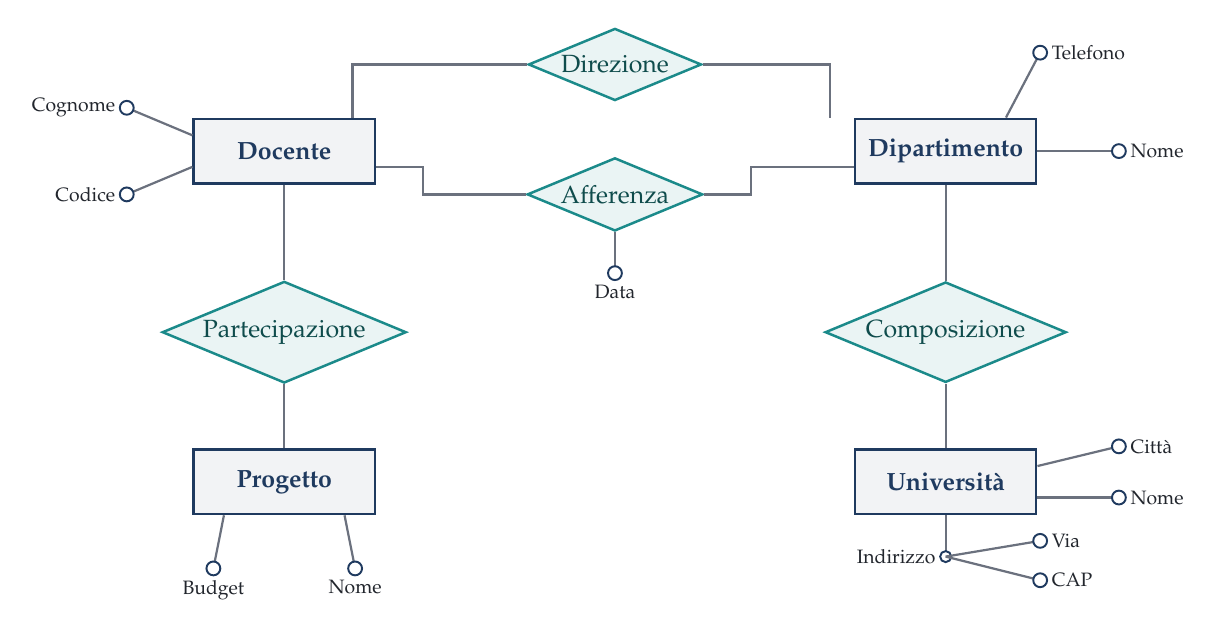
\begin{tikzpicture}[x=1cm,y=1cm]
    \node[ent] (D) at (0,0) {Docente};
    \node[ent] (Dip) at (8.4,0) {Dipartimento};
    \node[rel] (Dir) at (4.2,1.1) {Direzione};
    \node[rel] (Aff) at (4.2,-.55) {Afferenza};
    \node[rel] (Par) at (0,-2.3) {Partecipazione};
    \node[ent] (P) at (0,-4.2) {Progetto};
    \node[rel] (Com) at (8.4,-2.3) {Composizione};
    \node[ent] (U) at (8.4,-4.2) {Università};
    \draw[lk] (D.north east) ++(-.3,0) |- (Dir.west);
    \draw[lk] (Dir.east) -| ([xshift=-.3cm]Dip.north west);
    \draw[lk] ([yshift=-.2cm]D.east) -- ++(.6,0) |- (Aff.west);
    \draw[lk] (Aff.east) -- ++(.6,0) |- ([yshift=-.2cm]Dip.west);
    \draw[lk] (D) -- (Par) -- (P);
    \draw[lk] (Dip) -- (Com) -- (U);
    \attributo{(D.west)++(0,.2)}{(-2,.55)}{Cognome}{left}
    \attributo{(Aff.south)}{(4.2,-1.55)}{Data}{below}
    \attributo{(P.south west)++(.4,0)}{(-.9,-5.3)}{Budget}{below}
    \attributo{(Dip.north east)++(-.4,0)}{(9.6,1.25)}{Telefono}{right}
    \attributo{(U.east)++(0,.2)}{(10.6,-3.75)}{Città}{right}
    \draw[lk] (U.south) -- (8.4,-5.15);
    \node[att,minimum size=4pt] (ind) at (8.4,-5.15) {};
    \node[attl,left=2pt] at (ind) {Indirizzo};
    \attributo{(8.4,-5.15)}{(9.6,-4.95)}{Via}{right}
    \attributo{(8.4,-5.15)}{(9.6,-5.45)}{CAP}{right}
    \ifunicard
      \idattributo{(D.west)++(0,-.2)}{(-2,-.55)}{Codice}{left}
      \idattributo{(P.south east)++(-.4,0)}{(.9,-5.3)}{Nome}{below}
      \idattributo{(U.east)++(0,-.2)}{(10.6,-4.4)}{Nome}{right}
      \attributo{(Dip.east)}{(10.6,0)}{Nome}{right}
      % identificatore esterno: Nome + Università (via Composizione)
      \draw[idl] (10.25,.45) -- (10.25,-1.1) -- (8.4,-1.1);
      \node[iddot] at (10.25,.45) {};
      \node[card,left] at ($(D.north east)+(-.3,.55)$) {(0,1)};
      \node[card,right] at ($(Dip.north west)+(-.3,.55)$) {(1,1)};
      \node[card,above] at ($(D.east)+(.4,-.2)$) {(0,1)};
      \node[card,above] at ($(Dip.west)+(-.35,-.2)$) {(0,N)};
      \node[card,right] at (0,-1.05) {(0,N)};
      \node[card,right] at (0,-3.55) {(1,N)};
      \node[card,left] at (8.4,-1.4) {(1,1)};
      \node[card,left] at (8.4,-3.55) {(1,N)};
      \node[card,right] at (9.6,1.6) {(1,N)};
    \else
      \attributo{(D.west)++(0,-.2)}{(-2,-.55)}{Codice}{left}
      \attributo{(P.south east)++(-.4,0)}{(.9,-5.3)}{Nome}{below}
      \attributo{(U.east)++(0,-.2)}{(10.6,-4.4)}{Nome}{right}
      \attributo{(Dip.east)}{(10.6,0)}{Nome}{right}
    \fi
  \end{tikzpicture}}

\begin{document}
% ================= COPERTINA =================
\thispagestyle{empty}
\begin{tikzpicture}[remember picture,overlay]
  \fill[navy] (current page.north west) rectangle ([yshift=-15.5cm]current page.north east);
  \fill[teal] ([yshift=-15.5cm]current page.north west) rectangle ([yshift=-16.1cm]current page.north east);
  \node[anchor=north west,font=\headfont\small\bfseries,text=ambra] at ([xshift=2.3cm,yshift=-2.2cm]current page.north west) {BASI DI DATI \,·\, PROGETTAZIONE CONCETTUALE};
  \node[anchor=north west,font=\headblack\fontsize{44}{48}\selectfont,text=white,align=left] at ([xshift=2.2cm,yshift=-3.0cm]current page.north west) {Il modello\\[2pt]Entity-Relationship};
  \node[anchor=north west,font=\headlight\Large,text=white!85!teal,align=left] at ([xshift=2.3cm,yshift=-7.1cm]current page.north west) {Entità, relationship, attributi, cardinalità,\\identificatori e generalizzazioni};
  % motivo: uno schema E-R stilizzato
  \begin{scope}[shift={([xshift=2.4cm,yshift=-13.6cm]current page.north west)},scale=1.22,white]
    \foreach \x/\y in {0/1.6,5.2/1.6,10.4/1.6,5.2/-1.2}{
      \fill[white,opacity=.13,rounded corners=2pt] (\x,\y) rectangle ++(2.6,1.1);}
    \foreach \x/\y in {3.9/2.15,9.1/2.15,6.5/.75}{
      \fill[white,opacity=.22] (\x-.8,\y) -- (\x,\y+.5) -- (\x+.8,\y) -- (\x,\y-.5) -- cycle;}
    \draw[white,opacity=.35,line width=1pt] (2.6,2.15) -- (3.1,2.15) (4.7,2.15) -- (5.2,2.15) (7.8,2.15) -- (8.3,2.15) (9.9,2.15) -- (10.4,2.15) (6.5,1.6) -- (6.5,1.25) (6.5,.25) -- (6.5,-.1);
    \foreach \x in {.6,1.3,2.0}{\draw[white,opacity=.35] (\x,2.7) -- (\x,3.3); \fill[white,opacity=.6] (\x,3.3) circle (.09);}
    \fill[ambra] (.6,3.3) circle (.11);
    \draw[ambra,line width=1.3pt] (.6,3.3) -- (.6,3.65) -- (2.25,3.65) -- (2.25,2.15);
    \node[font=\headfont\bfseries\scriptsize,text=ambra,anchor=west] at (2.4,3.65) {identificatore};
  \end{scope}
\end{tikzpicture}
\vspace*{15.0cm}
\begin{center}
\begin{tcolorbox}[enhanced,width=.86\linewidth,colback=white,colframe=navy!35,arc=6pt,boxrule=.8pt,halign=flush center,top=6pt,bottom=6pt]
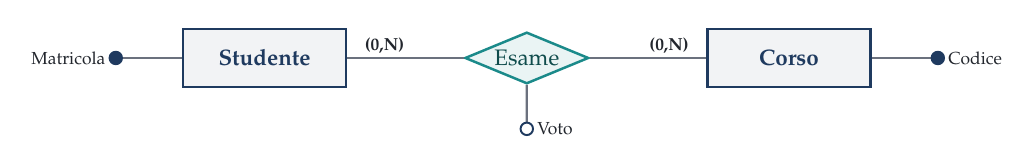
\begin{tikzpicture}[scale=.9,every node/.append style={transform shape}]
  \node[ent] (S) at (0,0) {Studente};
  \node[rel] (E) at (3.7,0) {Esame};
  \node[ent] (C) at (7.4,0) {Corso};
  \draw[lk] (S) -- (E) node[card,pos=.32,above]{(0,N)};
  \draw[lk] (E) -- (C) node[card,pos=.68,above]{(0,N)};
  \idattributo{(S.west)}{(-2.1,0)}{Matricola}{left}
  \idattributo{(C.east)}{(9.5,0)}{Codice}{right}
  \attributo{(E.south)}{(3.7,-1)}{Voto}{right}
\end{tikzpicture}\\[2pt]
{\headfont\small\color{grigio}descrivere \emph{che cosa} rappresentare, prima di decidere \emph{come}}
\end{tcolorbox}
\vspace{.7cm}
{\headfont\large\color{navy}\bfseries Manuale di studio\par}
\vspace{2pt}
{\headfont\color{grigio}\autore\par}
\vspace{.8cm}

\begin{tikzpicture}
  \foreach \c/\t [count=\i] in {teal/Intuizione,navy/Tecnica,ambra/Esempi,rosso/Attenzione,blu/Esercizi}{
    \node[fill=\c,text=white,font=\headfont\bfseries\footnotesize,rounded corners=3pt,minimum width=2.5cm,minimum height=.6cm] at (\i*2.85,0) {\t};}
\end{tikzpicture}
\end{center}
% ================= COME USARE =================
\clearpage\thispagestyle{plain}
{\headfont\bfseries\Huge\color{navy}Come usare questo manuale\par}
\vspace{4pt}{\color{teal}\rule{3cm}{2.5pt}}\vspace{8pt}

Il manuale segue le due lezioni sul modello Entity-Relationship (slide 1–102 e 103–157). I capitoli vanno letti in ordine: ogni costrutto usa quelli precedenti. Il capitolo sugli \hl{identificatori} (capitolo 6) è stato \key{ampliato} rispetto alle slide con la documentazione di riferimento: notazione grafica completa, identificatori composti e multipli, minimalità, il confronto con le «entità deboli» dei testi in inglese e un esercizio d'esame svolto passo per passo. Nei riepiloghi di fine capitolo le etichette verdi «p.\,$n$» indicano la slide corrispondente.

I riquadri hanno sempre lo stesso significato; ognuno ha un'icona e un titolo, quindi si riconosce anche stampato in bianco e nero.
\begin{intuizione}L'idea di fondo, con un esempio quotidiano.\end{intuizione}
\begin{tecnica}Definizioni precise e regole del modello.\end{tecnica}
\begin{esempio}Schemi e occorrenze svolti passo per passo.\end{esempio}
\begin{attenzione}Errori frequenti e punti in cui i testi usano convenzioni diverse.\end{attenzione}
\begin{consiglio}Abitudini utili quando si disegna uno schema.\end{consiglio}
\begin{mlbox}Collegamenti con altri argomenti del corso e approfondimenti.\end{mlbox}
\begin{esercizi}Esercizi di fine capitolo: le soluzioni sono in appendice.\end{esercizi}


% ================= INDICE =================
\clearpage\thispagestyle{plain}
\tableofcontents
\vspace{12pt}
\begin{mlbox}[Notazione usata]
Gli schemi seguono la notazione del libro di Atzeni, Ceri, Fraternali, Paraboschi e Torlone, la stessa delle slide: \key{rettangoli} per le entità, \key{rombi} per le relationship, \key{pallini} per gli attributi (pieni se formano un identificatore), coppie $(\min,\max)$ per le cardinalità, \key{frecce} per le generalizzazioni. Il riassunto di tutti i simboli è nella \hl{scheda della notazione} in fondo al manuale.
\end{mlbox}

\sezione{1}{Perché serve un modello concettuale}{slide 3–38}

\begin{inbreve}
Progettare una base di dati scrivendo subito le tabelle è come costruire una casa partendo dalle tubature: si finisce nei dettagli prima di aver capito che cosa serve. La \hl{progettazione concettuale} descrive prima i \key{concetti} della realtà di interesse e i loro legami, con un linguaggio grafico indipendente dal DBMS: il \hl{modello Entity-Relationship} (E-R).
\end{inbreve}

\subsection{Il problema: partire dalle tabelle}

\begin{intuizione}[La ricevuta del ristorante]
Una ricevuta fiscale ha un numero, una data, un totale e un elenco di righe (quantità, descrizione, importo). È una struttura \hl{nidificata}: dentro la ricevuta c'è una lista. Nel modello relazionale i valori devono essere \key{semplici}, non tabelle: la ricevuta va quindi spezzata in due relazioni, \emph{Ricevute} e \emph{Dettaglio}, collegate dal numero della ricevuta.
\end{intuizione}

\begin{center}
\small
\renewcommand{\arraystretch}{1.2}
\begin{minipage}[t]{.36\linewidth}\centering
{\headfont\bfseries\small\color{navy}Ricevute}\\[3pt]
\rowcolors{2}{chiaro}{white}
\begin{tabular}{lll}
\rowcolor{navy}\thd{Numero} & \thd{Data} & \thd{Totale}\\
1235 & 12/10/2019 & 39,20\\
1240 & 13/10/2019 & 39,00\\
\end{tabular}
\end{minipage}\hfill
\begin{minipage}[t]{.6\linewidth}\centering
{\headfont\bfseries\small\color{navy}Dettaglio}\\[3pt]
\rowcolors{2}{chiaro}{white}
\begin{tabular}{lllll}
\rowcolor{navy}\thd{Numero} & \thd{Riga} & \thd{Qtà} & \thd{Descrizione} & \thd{Importo}\\
1235 & 1 & 3 & Coperti & 3,00\\
1235 & 2 & 2 & Antipasti & 6,20\\
1235 & 3 & 3 & Primi & 12,00\\
1235 & 4 & 2 & Bistecche & 18,00\\
1240 & 1 & 2 & Coperti & 2,00\\
\end{tabular}
\end{minipage}
\end{center}
\didascalia{Due relazioni per una struttura nidificata (slide 14). La colonna \emph{Riga} serve solo se interessano l'ordine delle righe o righe ripetute.}

Perché due relazioni? Perché ci sono \hl{due concetti diversi}, con livelli di dettaglio diversi: la \key{ricevuta} e la \key{riga} della ricevuta. E che cosa rappresentare dipende da che cosa ci interessa: possono esistere righe ripetute? Conta l'ordine delle righe? A seconda delle risposte cambiano i dettagli (la colonna \emph{Riga}), ma \key{i concetti restano gli stessi}.

Partendo direttamente dallo schema logico si incontrano tre problemi: non si sa da dove cominciare, ci si perde subito nei dettagli (attributi, chiavi, vincoli di riferimento) e il modello relazionale è «rigido». Servono un \hl{metodo} (una metodologia di progettazione) e un \hl{modello} per rappresentare i concetti.

\subsection{La progettazione nel ciclo di vita}

La progettazione della base di dati è una delle attività del \hl{ciclo di vita dei sistemi informativi}: l'insieme ordinato delle attività svolte da analisti, progettisti e utenti per sviluppare e usare un sistema. È un ciclo perché le fasi si ripetono e non sono nettamente separate.

\begin{center}
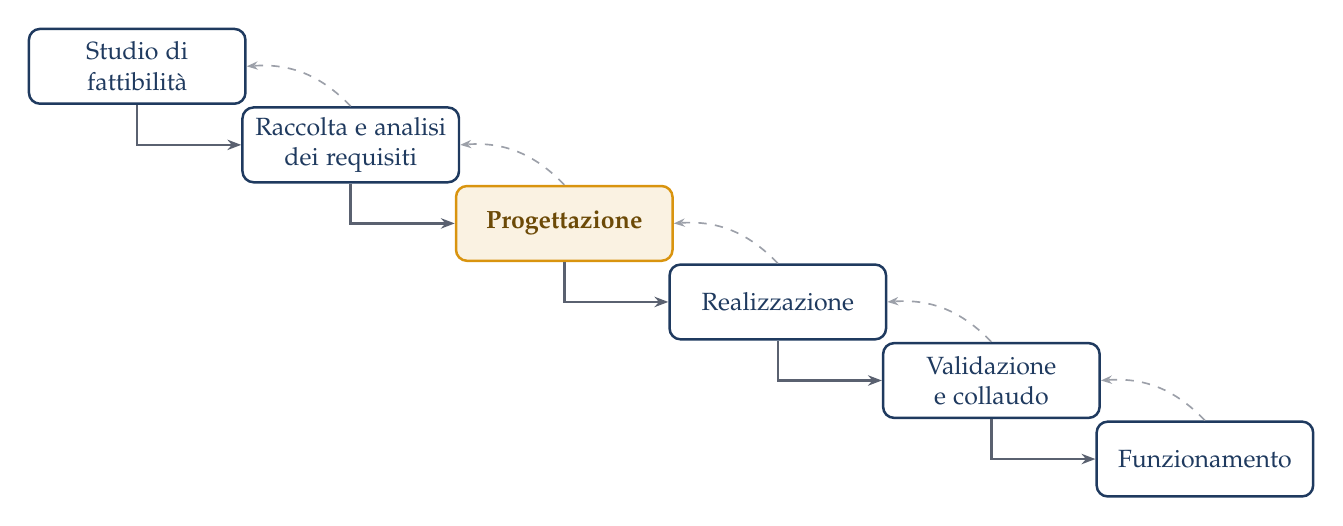
\begin{tikzpicture}[x=1.13cm,y=.95cm,
  fase/.style={draw=navy,fill=white,line width=.9pt,rounded corners=4pt,minimum width=2.75cm,minimum height=.95cm,align=center,font=\headfont\small,text=navy},
  fr/.style={-{Stealth[length=5pt]},line width=.9pt,color=grigio},
  rit/.style={-{Stealth[length=4pt]},line width=.6pt,color=grigio!60,dashed}]
  \node[fase] (a) at (0,0) {Studio di\\fattibilità};
  \node[fase] (b) at (2.4,-1.05) {Raccolta e analisi\\dei requisiti};
  \node[fase,draw=ambra,fill=ambra!12,text=ambra!50!black] (c) at (4.8,-2.1) {\textbf{Progettazione}};
  \node[fase] (d) at (7.2,-3.15) {Realizzazione};
  \node[fase] (e) at (9.6,-4.2) {Validazione\\e collaudo};
  \node[fase] (f) at (12.0,-5.25) {Funzionamento};
  \foreach \u/\v in {a/b,b/c,c/d,d/e,e/f}{\draw[fr] (\u.south) |- (\v.west);}
  \foreach \u/\v in {b/a,c/b,d/c,e/d,f/e}{\draw[rit] (\u.north) to[bend right=25] (\v.east);}
\end{tikzpicture}
\end{center}
\didascalia{Il ciclo di vita (slide 18): le frecce tratteggiate indicano che si può tornare alle fasi precedenti.}

\begin{center}
\small
\renewcommand{\arraystretch}{1.3}\renewcommand\tabularxcolumn[1]{m{#1}}
\rowcolors{2}{chiaro}{white}
\begin{tabularx}{.92\linewidth}{>{\raggedright\headfont\bfseries\small}m{4.4cm} >{\raggedright\arraybackslash}X}
\rowcolor{navy}\thd{Fase} & \thd{In che cosa consiste}\\
Studio di fattibilità & Definizione di costi e priorità.\\
Raccolta e analisi dei requisiti & Studio delle proprietà che il sistema deve avere.\\
Progettazione & Progettazione dei \key{dati} e delle \key{funzioni}.\\
Realizzazione & Costruzione del sistema.\\
Validazione e collaudo & Sperimentazione per verificare che funzioni come previsto.\\
Funzionamento & Il sistema diventa operativo.\\
\end{tabularx}
\end{center}

In questo corso ci concentriamo sulla \hl{progettazione dei dati}: i dati hanno un ruolo centrale e sono \key{più stabili} delle applicazioni che li usano.

\subsection{Le tre fasi della progettazione dei dati}

\begin{center}
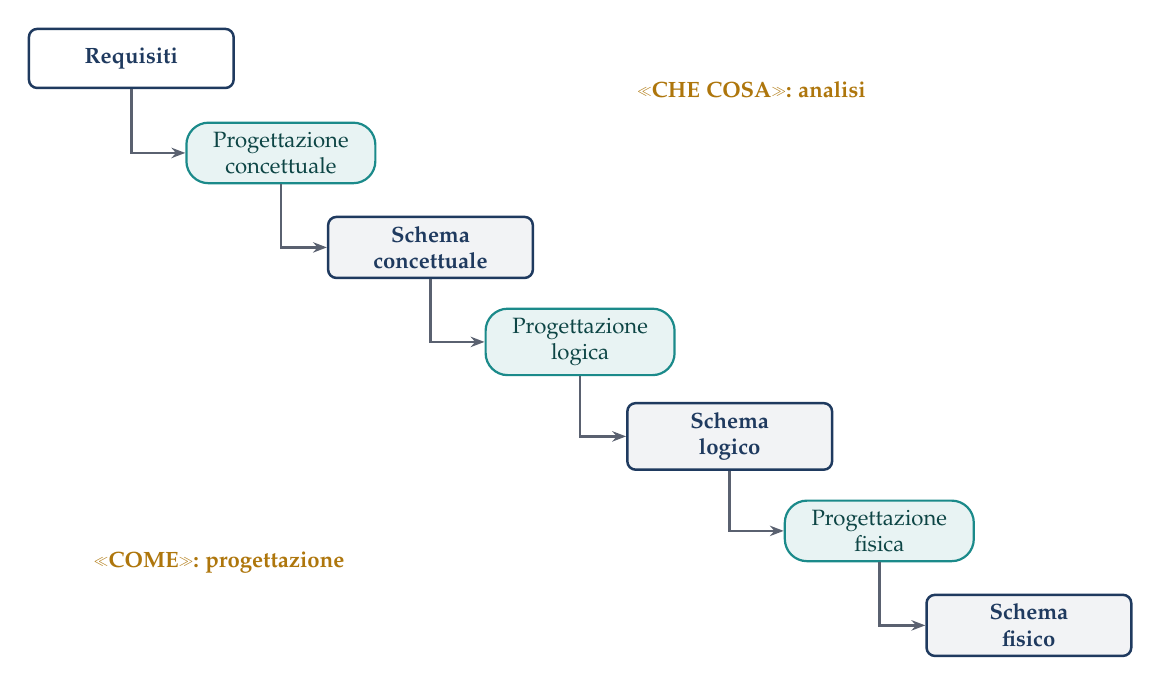
\begin{tikzpicture}[x=1cm,y=1cm,
  prod/.style={draw=navy,fill=navy!6,line width=.9pt,rounded corners=3pt,minimum width=2.6cm,minimum height=.75cm,font=\headfont\bfseries\footnotesize,text=navy,align=center},
  att/.style={draw=teal,fill=teal!10,line width=.8pt,rounded corners=8pt,minimum width=2.4cm,minimum height=.75cm,font=\headfont\footnotesize,text=teal!50!black,align=center},
  fr/.style={-{Stealth[length=5pt]},line width=.9pt,color=grigio}]
  \node[prod,fill=white] (r) at (0,0) {Requisiti};
  \node[att] (pc) at (1.9,-1.2) {Progettazione\\concettuale};
  \node[prod] (sc) at (3.8,-2.4) {Schema\\concettuale};
  \node[att] (pl) at (5.7,-3.6) {Progettazione\\logica};
  \node[prod] (sl) at (7.6,-4.8) {Schema\\logico};
  \node[att] (pf) at (9.5,-6.0) {Progettazione\\fisica};
  \node[prod] (sf) at (11.4,-7.2) {Schema\\fisico};
  \foreach \u/\v in {r/pc,pc/sc,sc/pl,pl/sl,sl/pf,pf/sf}{\draw[fr] (\u.south) |- (\v.west);}
  \node[font=\headfont\bfseries\footnotesize,text=ambra!80!black,align=left,anchor=west] at (6.3,-.4) {«CHE COSA»: analisi};
  \node[font=\headfont\bfseries\footnotesize,text=ambra!80!black,align=left,anchor=west] at (-.6,-6.4) {«COME»: progettazione};
\end{tikzpicture}
\end{center}
\didascalia{Dai requisiti agli schemi (slide 23–25). Ogni fase produce uno schema in un modello dei dati diverso.}

\begin{tecnica}[Prodotti della progettazione]
\begin{itemize}
  \item \hl{Schema concettuale}: descrive \emph{che cosa} rappresentare, con il modello E-R.
  \item \hl{Schema logico}: descrive i dati nel modello del DBMS scelto (ad esempio relazionale).
  \item \hl{Schema fisico}: descrive come i dati sono memorizzati (file, indici).
\end{itemize}
Un \key{modello dei dati} è un insieme di costrutti, cioè un «linguaggio» per rappresentare ciò che interessa: il modello relazionale, per esempio, ha come costrutto la relazione (tabella).
\end{tecnica}

\subsection{Modelli logici e modelli concettuali}

\begin{center}
\small
\renewcommand{\arraystretch}{1.35}\renewcommand\tabularxcolumn[1]{m{#1}}
\rowcolors{2}{chiaro}{white}
\begin{tabularx}{\linewidth}{>{\raggedright\arraybackslash}X >{\raggedright\arraybackslash}X}
\rowcolor{navy}\thd{Modello logico (es. relazionale)} & \thd{Modello concettuale (E-R)}\\
Rappresenta i dati come tabelle & Rappresenta i concetti del dominio (la realtà di interesse)\\
Dipende dal tipo di DBMS & Indipendente dal DBMS\\
Si scrive in SQL con \texttt{CREATE TABLE} & Si disegna: è pensato per essere letto da tutti, anche dai non informatici\\
Si ottiene traducendo lo schema E-R & Non descrive come si accede ai dati\\
Esempi: relazionale, reticolare, a oggetti, XML, NoSQL & Il più noto e diffuso: Entity-Relationship\\
\end{tabularx}
\end{center}

\begin{mlbox}[Da dove viene il modello E-R]
Il modello Entity-Relationship è stato proposto da Peter Chen nel 1976, nell'articolo \emph{The Entity-Relationship Model – Toward a Unified View of Data} (ACM Transactions on Database Systems). Ne esistono molte versioni, più o meno diverse tra loro: questo manuale usa quella del libro di Atzeni e colleghi, adottata nel corso.
\end{mlbox}

Il filo conduttore degli esempi è l'\hl{università}: una realtà che conosciamo tutti «dall'interno» e che contiene molti concetti collegati in modi diversi (studenti, corsi, docenti, esami, corsi di laurea, dipartimenti, aule, progetti).

\begin{tecnica}[I costrutti del modello E-R]
Entità, relationship, attributi, cardinalità (di relationship e di attributo), identificatori (interni ed esterni), generalizzazioni. I prossimi capitoli li presentano uno alla volta.
\end{tecnica}

\begin{esercizi}
\begin{passi}
  \item Indica per ciascuna affermazione se riguarda il modello logico o quello concettuale: (a) dipende dal DBMS; (b) può essere discusso con un committente non informatico; (c) contiene vincoli di chiave esterna.
  \item Nella ricevuta del ristorante, quale informazione rende necessaria la colonna \emph{Riga}?
\end{passi}
\end{esercizi}

\begin{appunti}{Riepilogo del capitolo}
\pag{9} Le strutture nidificate non sono ammesse nel relazionale: si spezzano in più relazioni.
\pag{11} Due relazioni perché ci sono due concetti diversi (ricevuta, riga).
\pag{16} Servono un metodo e un modello per non perdersi nei dettagli.
\pag{23} Progettazione concettuale (che cosa) → logica → fisica (come).
\pag{31} Modello concettuale: indipendente dal DBMS, leggibile da tutti.
\end{appunti}

\sezione{2}{Entità}{slide 38–48}

\begin{inbreve}
Un'\hl{entità} rappresenta una classe di oggetti della realtà di interesse (persone, cose, fatti) con proprietà comuni ed esistenza autonoma. Nello schema si disegna come un \key{rettangolo} con il nome dentro. Lo schema rappresenta le classi, non i singoli oggetti.
\end{inbreve}

\subsection{Definizione}

\begin{tecnica}[Entità]
Classe di oggetti (fatti, persone, cose) della realtà di interesse con \hl{proprietà comuni} e con \hl{esistenza «autonoma»}, nel senso che i singoli oggetti sono in qualche modo riconoscibili.

Esempi: studente, docente, corso, aula, dipartimento.
\end{tecnica}

\par\noindent\begin{minipage}{\linewidth}
\begin{schema}[x=1cm]
  \foreach \x/\n in {0/Studente,3/Docente,6/Corso,9/Aula,12/Dipartimento}{\node[ent,minimum width=2.4cm] at (\x,0) {\n};}
\end{schema}
\didascalia{Rappresentazione grafica delle entità: un rettangolo con il nome (slide 44).}
\end{minipage}\par

\subsection{Schema e istanza}

\begin{intuizione}[Lo stampo e i biscotti]
L'entità è lo \hl{stampo}: dice che forma hanno tutti gli studenti. Le \key{occorrenze} sono i biscotti: Mario Rossi, Piero Neri e così via. Lo schema concettuale disegna gli stampi, non i biscotti.
\end{intuizione}

\begin{tecnica}[Entità e occorrenza]
\begin{itemize}
  \item \hl{Entità}: classe di oggetti, persone, … «omogenei».
  \item \hl{Occorrenza} di entità: un elemento della classe, cioè \key{l'oggetto o la persona stessa}, non i dati che la descrivono.
  \item Nello schema concettuale si rappresentano le entità, non le singole occorrenze: è un'\key{astrazione}.
\end{itemize}
\end{tecnica}

\begin{attenzione}[Occorrenza non è riga]
Un'occorrenza è la persona Mario Rossi, non la riga di una tabella che contiene i suoi dati. Nel modello relazionale ogni riga «rappresenta» un oggetto; nel modello E-R l'occorrenza \emph{è} l'oggetto. La distinzione aiuta a capire perché due occorrenze diverse possono avere valori uguali per alcuni attributi (due studenti omonimi).
\end{attenzione}

\subsection{Quali entità? L'esempio della biblioteca}

Le specifiche dell'esercizio d'esame del 13/09/2002 (lo risolveremo per intero nel capitolo 9) parlano di prestiti di «libri». Ma che cosa è un libro? Proviamo a chiederci quali sarebbero le \hl{occorrenze} di un'entità \emph{Libro}:
\begin{itemize}
  \item le \key{opere} («I Miserabili» di Victor Hugo)?
  \item le \key{edizioni} (Mondadori, collana Oscar, 1975)?
  \item i \key{volumi} (il terzo volume di quell'edizione)?
  \item le \key{copie} (la seconda copia di quel volume, che sta sullo scaffale)?
\end{itemize}

\par\noindent\begin{minipage}{\linewidth}
\begin{schema}[x=1cm]
  \node[ent] at (0,0) {Opera};
  \node[ent] at (3.2,0) {Edizione};
  \node[ent] at (6.4,0) {Volume};
  \node[ent] at (9.6,0) {Copia};
\end{schema}
\didascalia{Probabilmente quattro entità diverse (slide 47): ognuna ha occorrenze diverse.}
\end{minipage}\par

\begin{esempio}[Contare le occorrenze]
Una biblioteca possiede 2 copie del terzo volume de «I Miserabili» (edizione Mondadori Oscar 1975, in 4 volumi) e 1 copia di ciascuno degli altri tre volumi. Allora ci sono: 1 opera, 1 edizione, 4 volumi e $2+3\cdot1=5$ copie. Un'unica entità \emph{Libro} non saprebbe dire «quanti libri» ci sono: 1, 4 o 5? Il fatto che le risposte siano diverse è il segnale che i concetti sono diversi.
\end{esempio}

\subsection{Convenzioni sui nomi}

\begin{consiglio}[Nomi delle entità]
Ogni entità ha un nome che la identifica \hl{univocamente} nello schema. Usa nomi \key{espressivi} e convenzioni uniformi: nomi al \key{singolare} (\emph{Studente}, non \emph{Studenti}), perché il nome descrive la classe, cioè com'è fatta ciascuna occorrenza.
\end{consiglio}

\begin{esercizi}
\begin{passi}
  \item In una realtà ospedaliera, quali entità useresti per «letto», «reparto», «ricovero»? Ricovero è un'entità o un legame tra altre entità?
  \item Perché \emph{Studenti} non è un buon nome di entità?
\end{passi}
\end{esercizi}

\begin{appunti}{Riepilogo del capitolo}
\pag{39} Entità = classe di oggetti con proprietà comuni ed esistenza autonoma.
\pag{43} Entità (classe) $\neq$ occorrenza (l'oggetto, non i dati).
\pag{47} Un «libro» può essere opera, edizione, volume o copia: concetti diversi.
\pag{48} Nomi espressivi, al singolare, unici nello schema.
\end{appunti}

\sezione{3}{Relationship}{slide 49–78}

\begin{inbreve}
Una \hl{relationship} è un legame logico fra due o più entità, rilevante per l'applicazione. Si disegna come un \key{rombo} collegato alle entità coinvolte. Le sue occorrenze sono \key{coppie} (o $n$-uple) di occorrenze di entità e, essendo un insieme, \hl{non possono ripetersi}: quando lo stesso legame può presentarsi più volte, la relationship va «promossa» a entità.
\end{inbreve}

\subsection{Definizione e rappresentazione}

\begin{tecnica}[Relationship]
Legame logico fra due o più entità, rilevante nell'applicazione di interesse. Esempi: \emph{Iscrizione} (fra studente e corso di laurea), \emph{Esame} (fra studente e corso). Si chiama anche relazione, correlazione o associazione.
\end{tecnica}

\par\noindent\begin{minipage}{\linewidth}
\begin{schema}
  \node[ent] (S) at (0,0) {Studente};
  \node[rel] (E) at (3.8,0) {Esame};
  \node[ent] (C) at (7.6,0) {Corso};
  \draw[lk] (S) -- (E) -- (C);
  \node[ent] (S2) at (0,-1.6) {Studente};
  \node[rel] (I) at (3.8,-1.6) {Iscrizione};
  \node[ent] (L) at (7.6,-1.6) {Corso di laurea};
  \draw[lk] (S2) -- (I) -- (L);
\end{schema}
\didascalia{Rappresentazione grafica di relationship (slide 50).}
\end{minipage}\par

\begin{consiglio}[Nomi delle relationship]
Come per le entità: nomi espressivi, unici nello schema, al singolare; \hl{sostantivi invece che verbi} quando possibile (\emph{Iscrizione} invece di \emph{si iscrive}). Un sostantivo non suggerisce un «verso» di lettura, mentre la relationship non ne ha.
\end{consiglio}

\subsection{Occorrenze di una relationship}

\begin{tecnica}[Occorrenze]
Un'occorrenza di una relationship \hl{binaria} è una \key{coppia} di occorrenze di entità, una per ciascuna entità coinvolta. Una relationship ha un \key{insieme} di occorrenze: quindi al suo interno \hl{non ci possono essere coppie ripetute}.
\end{tecnica}

\par\noindent\begin{minipage}{\linewidth}
\begin{schema}[x=1cm,y=1cm]
  \node[insieme,minimum width=1.6cm,minimum height=3.8cm] at (0,0) {};
  \node[insieme,minimum width=1.9cm,minimum height=3.8cm] at (4,0) {};
  \node[insieme,minimum width=1.6cm,minimum height=3.8cm] at (8,0) {};
  \foreach \n/\y in {S1/1.2,S2/.4,S3/-.4,S4/-1.2}{\node[occ] (\n) at (0,\y){}; \node[occl,left] at (\n){\n};}
  \foreach \n/\y in {C1/1.0,C2/0,C3/-1.0}{\node[occ] (\n) at (8,\y){}; \node[occl,right] at (\n){\n};}
  \foreach \n/\y/\a/\b in {e1/1.2/S1/C1,e2/.4/S2/C1,e3/-.4/S2/C2,e4/-1.2/S4/C3}{
    \node[occ,fill=teal] (\n) at (4,\y){};
    \draw[lk,line width=.5pt] (\a) -- (\n) -- (\b);}
  \foreach \n/\t in {e1/{(S1,C1)},e2/{(S2,C1)},e3/{(S2,C2)},e4/{(S4,C3)}}{\node[occl,fill=chiaro,above=2pt] at (\n) {\t};}
  \node[font=\headfont\bfseries\small,text=navy] at (0,-2.3) {Studente};
  \node[font=\headfont\bfseries\small,text=teal] at (4,-2.3) {Esame};
  \node[font=\headfont\bfseries\small,text=navy] at (8,-2.3) {Corso};
\end{schema}
\didascalia{Occorrenze della relationship Esame (slide 52): ogni occorrenza è una coppia (studente, corso). S3 non ha esami; C2 e C3 ne hanno uno ciascuno.}
\end{minipage}\par

\subsection{Quando la relationship non basta: promuoverla a entità}

\begin{intuizione}[Mourinho al Real Madrid]
Proviamo a rappresentare gli allenatori delle squadre con la relationship \emph{Incarico} fra \emph{Squadra} e \emph{Allenatore}. José Mourinho ha allenato il Real Madrid due volte, in periodi diversi. Ma la coppia (Real Madrid, Mourinho) può comparire \hl{una sola volta} nell'insieme delle occorrenze: il secondo incarico non si può registrare.
\end{intuizione}

\par\noindent\begin{minipage}{\linewidth}
\begin{schema}[x=1cm,y=1cm]
  \node[ent] (Q) at (0,0) {Squadra};
  \node[rel] (Inc) at (3.6,0) {Incarico};
  \node[ent] (A) at (7.2,0) {Allenatore};
  \draw[lk] (Q) -- (Inc) -- (A);
  \draw[-{Stealth[length=7pt]},line width=2pt,ambra] (3.6,-.65) -- (3.6,-1.25);
  \node[ent] (Q2) at (-1.2,-1.9) {Squadra};
  \node[rel,minimum width=1.5cm,minimum height=.75cm] (R1) at (1.25,-1.9) {};
  \node[ent] (Inc2) at (3.6,-1.9) {Incarico};
  \node[rel,minimum width=1.5cm,minimum height=.75cm] (R2) at (5.95,-1.9) {};
  \node[ent] (A2) at (8.4,-1.9) {Allenatore};
  \draw[lk] (Q2) -- (R1) -- (Inc2) -- (R2) -- (A2);
  \node[nota] at (3.6,-2.75) {la relationship diventa un'entità, collegata da due nuove relationship};
\end{schema}
\didascalia{«Promuovere» la relationship a entità (slide 62). Ogni incarico diventa un oggetto a sé: due incarichi della stessa coppia sono due occorrenze diverse.}
\end{minipage}\par

\begin{tecnica}[Regola pratica]
Se la \hl{stessa coppia} di occorrenze può legarsi \key{più volte} (incarichi ripetuti, esami ripetuti, visite ripetute dallo stesso medico), la relationship \hl{non basta}: il legame va rappresentato con un'\key{entità}, collegata alle entità originarie. Vale la stessa domanda per \emph{Esame} fra Studente e Corso (uno studente può ripetere l'esame?) e per \emph{Visita} fra Paziente e Medico.
\end{tecnica}

\subsection{Relationship $n$-arie}

\begin{tecnica}[Occorrenze di una relationship $n$-aria]
Un'occorrenza di una relationship $n$-aria è una \key{$n$-upla} di occorrenze di entità, una per ciascuna entità coinvolta. Anche qui non ci possono essere $n$-uple ripetute.
\end{tecnica}

\par\noindent\begin{minipage}{\linewidth}
\begin{schema}
  \node[ent] (D) at (0,0) {Docente};
  \node[rel] (L) at (3.8,0) {Lezione};
  \node[ent] (C) at (7.6,0) {Corso};
  \node[ent] (A) at (3.8,-1.7) {Aula};
  \draw[lk] (D) -- (L) -- (C); \draw[lk] (L) -- (A);
\end{schema}
\didascalia{Relationship ternaria (slide 66): ogni occorrenza è una terna (docente, corso, aula).}
\end{minipage}\par

\begin{attenzione}[Quando è corretta la ternaria?]
Lo schema dice che una terna (docente, corso, aula) compare \hl{al più una volta}. Se per «lezione» intendiamo il singolo incontro (il docente D1 tiene il corso C1 nell'aula A1 \emph{ogni martedì}), le lezioni ripetute nella stessa aula non sono rappresentabili. Se invece «lezione» indica \key{dove} un docente tiene un corso, lo schema va bene. Prima di disegnare chiediti sempre \emph{che cosa} è un'occorrenza.
\end{attenzione}

\subsection{Più relationship sulle stesse entità}

Fra le stesse entità possono esistere più relationship, con significati diversi:

\par\noindent\begin{minipage}{\linewidth}
\begin{schema}
  \node[ent] (S) at (0,0) {Studente};
  \node[rel] (Res) at (3.8,0) {Residenza};
  \node[ent] (C) at (7.6,0) {Città};
  \node[rel] (N) at (3.8,1.35) {Nascita};
  \draw[lk] (S) -- (Res) -- (C);
  \draw[lk] (S.north) |- (N.west); \draw[lk] (N.east) -| (C.north);
\end{schema}
\didascalia{Nascita e Residenza collegano entrambe Studente e Città (slide 72).}
\end{minipage}\par

\subsection{Relationship ricorsive e ruoli}

\begin{tecnica}[Relationship ricorsiva]
Coinvolge \hl{«due volte» la stessa entità}. Esempio: \emph{Collaborazione} fra docenti. Quando i due «posti» del legame hanno significati diversi, si indicano i \key{ruoli}: in \emph{Propedeuticità} su \emph{Corso} un corso partecipa come \emph{Propedeutico}, l'altro come \emph{Successivo} («Basi di dati 1 è propedeutico a Basi di dati 2»).
\end{tecnica}

\par\noindent\begin{minipage}{\linewidth}
\begin{schema}[x=1cm,y=1cm]
  \node[ent] (D) at (0,0) {Docente};
  \node[rel] (Co) at (0,1.5) {Collaborazione};
  \draw[lk] (D.west) -- ++(-.8,0) |- (Co.west);
  \draw[lk] (D.east) -- ++(.8,0) |- (Co.east);
  \node[ent] (C) at (7,0) {Corso};
  \node[rel] (P) at (9.4,1.5) {Propedeuticità};
  \draw[lk] (C.north) |- (P.west) node[pos=.25,left,font=\headfont\scriptsize\itshape,text=teal]{Propedeutico};
  \draw[lk] (C.east) -| (P.south) node[pos=.3,below,font=\headfont\scriptsize\itshape,text=teal]{Successivo};
\end{schema}
\didascalia{Relationship ricorsive senza ruoli (a sinistra) e con ruoli (a destra), slide 73–74.}
\end{minipage}\par

\begin{esempio}[Occorrenze con ruoli]
Con i corsi C1, C2, C3, le occorrenze di \emph{Propedeuticità} possono essere P1 = (Propedeutico: C1, Successivo: C2) e P2 = (Propedeutico: C2, Successivo: C3). Il corso C2 compare in entrambe, ma con \hl{ruoli diversi}.
\end{esempio}

\begin{attenzione}[La successione fra sovrani]
\emph{Successione} su \emph{Sovrano}, con ruoli \emph{Predecessore} e \emph{Successore}, è corretta? Se un sovrano può regnare in periodi non consecutivi (abdica e poi torna sul trono), la stessa coppia (predecessore, successore) può ripetersi, oppure servono informazioni sul periodo. In quel caso conviene \hl{promuovere \emph{Successione} a entità}, collegata due volte a \emph{Sovrano} (slide 78).
\end{attenzione}

\begin{esercizi}
\begin{passi}
  \item Un paziente può essere visitato più volte dallo stesso medico. Disegna uno schema corretto per le visite.
  \item Rappresenta la relationship «è sposato con» fra persone. Servono i ruoli?
\end{passi}
\end{esercizi}

\begin{appunti}{Riepilogo del capitolo}
\pag{49} Relationship = legame logico fra due o più entità; rombo; nome sostantivo singolare.
\pag{53} Occorrenze = coppie ($n$-uple); è un insieme: niente ripetizioni.
\pag{62} Legami ripetuti fra la stessa coppia ⇒ promuovere la relationship a entità.
\pag{65} Relationship $n$-arie: occorrenze $n$-uple.
\pag{73} Ricorsive: la stessa entità due volte; ruoli se i posti hanno significati diversi.
\end{appunti}

\sezione{4}{Attributi}{slide 81–86 e 101–102}

\begin{inbreve}
Un \hl{attributo} è una proprietà elementare di un'entità o di una relationship. Associa a ogni occorrenza un valore preso da un \key{dominio}. Si disegna come un pallino collegato al costrutto che descrive. Gli attributi possono essere \key{composti} e avere una \key{cardinalità} che indica opzionalità o valori multipli.
\end{inbreve}

\subsection{Definizione}

\begin{tecnica}[Attributo]
Proprietà \hl{elementare} di un'entità o di una relationship, di interesse ai fini dell'applicazione. Associa a ogni occorrenza di entità o di relationship un valore appartenente a un insieme detto \key{dominio} dell'attributo.
\end{tecnica}

\par\noindent\begin{minipage}{\linewidth}
\begin{schema}
  \node[ent] (S) at (0,0) {Studente};
  \node[rel] (E) at (4.2,0) {Esame};
  \node[ent] (C) at (8.4,0) {Corso};
  \draw[lk] (S) -- (E) -- (C);
  \attributo{(-.7,.41)}{(-1.3,1.3)}{Matricola}{above}
  \attributo{(0,.41)}{(0,1.3)}{Cognome}{above}
  \attributo{(.7,.41)}{(1.3,1.3)}{Nome}{above}
  \attributo{(E.south)}{(3.6,-1.2)}{Data}{below}
  \attributo{(E.south)}{(4.8,-1.2)}{Voto}{below}
  \attributo{(8.0,.41)}{(7.6,1.3)}{Codice}{above}
  \attributo{(8.8,.41)}{(9.2,1.3)}{Titolo}{above}
\end{schema}
\didascalia{Attributi di entità e di relationship (slide 82). Data e Voto descrivono il singolo esame, cioè la coppia (studente, corso).}
\end{minipage}\par

\begin{esempio}[Occorrenze con i valori degli attributi]
\begin{itemize}
  \item Studente S1: Matricola 34567, Cognome Rossi, Nome Mario.
  \item Corso C1: Codice Inf205, Titolo Basi di dati.
  \item Esame E1 = (S1, C1): Data 25/07/2004, Voto 26.
\end{itemize}
Il voto non è una proprietà dello studente (ne ha uno per ogni esame) né del corso (ne ha uno per ogni studente): è una proprietà del \hl{legame}, quindi è un attributo della relationship.
\end{esempio}

\subsection{Attributi composti}

\begin{tecnica}[Attributo composto]
Raggruppa attributi della stessa entità o relationship che hanno affinità di significato o di uso. Esempio: \emph{Via}, \emph{Numero civico} e \emph{CAP} formano un \emph{Indirizzo}. Nel corso si usano poco (quasi per niente).
\end{tecnica}

\par\noindent\begin{minipage}{\linewidth}
\begin{schema}
  \node[ent] (S) at (0,0) {Studente};
  \attributo{(S.north)}{(0,1.1)}{Cognome}{above}
  \attributo{(S.west)}{(-1.9,0)}{Età}{left}
  \draw[lk] (S.east) -- (2.6,0);
  \node[draw=navy,ellipse,fill=white,line width=.7pt,font=\headfont\scriptsize,inner sep=1.5pt] (I) at (3.3,0) {Indirizzo};
  \attributo{(I.east)}{(5.2,.6)}{Via}{right}
  \attributo{(I.east)}{(5.2,0)}{Numero}{right}
  \attributo{(I.east)}{(5.2,-.6)}{CAP}{right}
\end{schema}
\didascalia{Attributo composto (slide 85): Indirizzo raggruppa Via, Numero e CAP.}
\end{minipage}\par

\subsection{Cardinalità degli attributi}

\begin{tecnica}[Cardinalità di attributo]
A un attributo si può associare una coppia $(\min,\max)$, con due scopi:
\begin{itemize}
  \item indicare l'\hl{opzionalità} («informazione incompleta»): minimo 0;
  \item indicare attributi \hl{multivalore}: massimo N (nel corso si usano pochissimo).
\end{itemize}
Se la cardinalità non è indicata vale $(1,1)$: ogni occorrenza ha esattamente un valore.
\end{tecnica}

\par\noindent\begin{minipage}{\linewidth}
\begin{schema}
  \node[ent] (S) at (0,0) {Studente};
  \attributo{(S.east)}{(3,.8)}{Telefono}{right}
  \attributo{(S.east)}{(3,0)}{Nome}{right}
  \attributo{(S.east)}{(3,-.8)}{Numero patente}{right}
  \node[card] at (2.1,.85) {(0,N)};
  \node[card] at (2.1,-.85) {(0,1)};
\end{schema}
\didascalia{Telefono: zero o più numeri; Nome: esattamente uno; Numero patente: facoltativo (slide 102).}
\end{minipage}\par

\subsection{Lo schema dell'università}

Mettendo insieme entità, relationship e attributi si ottiene uno schema completo. Lo riprenderemo con le cardinalità e gli identificatori.

\par\noindent\begin{minipage}{\linewidth}
\begin{center}\schemauniversita{false}\end{center}
\didascalia{Schema dell'università con entità, relationship e attributi (slide 86).}
\end{minipage}\par

\begin{esercizi}
\begin{passi}
  \item Nello schema dell'università, dove metteresti l'attributo «data di inizio della direzione»? E «budget del progetto»?
  \item Rappresenta un'entità \emph{Persona} con un indirizzo email obbligatorio e un secondo indirizzo facoltativo.
\end{passi}
\end{esercizi}

\begin{appunti}{Riepilogo del capitolo}
\pag{81} Attributo = proprietà elementare; valori in un dominio.
\pag{82} Anche le relationship hanno attributi (Data, Voto di Esame).
\pag{84} Attributi composti: raggruppano attributi affini (poco usati).
\pag{101} Cardinalità di attributo: $(0,1)$ opzionale, $(0,N)$ o $(1,N)$ multivalore; default $(1,1)$.
\end{appunti}

\sezione{5}{Cardinalità delle relationship}{slide 87–100}

\begin{inbreve}
Le \hl{cardinalità} dicono a quante occorrenze di una relationship può partecipare ciascuna occorrenza di un'entità: una coppia $(\min,\max)$ scritta \key{accanto all'entità} a cui si riferisce. Dalle cardinalità massime si distinguono relationship \key{uno a uno}, \key{uno a molti} e \key{molti a molti}.
\end{inbreve}

\subsection{Definizione}

\begin{tecnica}[Cardinalità di relationship]
Coppia di valori associata a ogni entità che partecipa a una relationship. Specifica il numero \hl{minimo} e \hl{massimo} di occorrenze della relationship a cui ciascuna occorrenza dell'entità può partecipare.
\end{tecnica}

\par\noindent\begin{minipage}{\linewidth}
\begin{schema}
  \node[ent] (S) at (0,0) {Studente};
  \node[rel] (F) at (4.2,0) {Frequenza};
  \node[ent] (C) at (8.4,0) {Corso};
  \draw[lk] (S) -- (F) node[card,pos=.3,above]{(2,5)};
  \draw[lk] (F) -- (C) node[card,pos=.7,above]{(0,50)};
  \node[nota] at (4.2,-1) {ogni studente frequenta da 2 a 5 corsi; ogni corso ha al massimo 50 frequentanti};
\end{schema}
\didascalia{Un esempio di cardinalità (un po' forzato), slide 89.}
\end{minipage}\par

\begin{intuizione}[Come leggere la cardinalità]
Mettiti \hl{nei panni di una singola occorrenza} dell'entità vicina alla coppia e chiediti: «a quanti legami di questo tipo partecipo, al minimo e al massimo?». La coppia $(2,5)$ accanto a Studente si legge: «ogni studente partecipa ad almeno 2 e al più 5 frequenze».
\end{intuizione}

\begin{tecnica}[I valori che usiamo]
Per semplicità si usano solo tre simboli:
\begin{itemize}
  \item \key{minimo}: 0 = partecipazione \hl{opzionale}; 1 = partecipazione \hl{obbligatoria};
  \item \key{massimo}: 1 oppure N (nessun limite).
\end{itemize}
\end{tecnica}

\subsection{Uno a uno, uno a molti, molti a molti}

Con riferimento alle cardinalità \key{massime} si hanno relationship \hl{uno a uno} (entrambi i massimi 1), \hl{uno a molti} (un massimo 1 e l'altro N), \hl{molti a molti} (entrambi N).

\par\noindent\begin{minipage}{\linewidth}
\begin{schema}[y=1.35cm]
  \foreach \y/\a/\r/\b/\ca/\cb in {0/Studente/Relatore/Docente/{(0,1)}/{(0,N)},-1/Studente/Iscrizione/Corso di laurea/{(1,1)}/{(0,N)},-2/Docente/Afferenza/Dipartimento/{(1,1)}/{(1,N)}}{
    \node[ent] (A) at (0,\y) {\a}; \node[rel] (R) at (4.2,\y) {\r}; \node[ent] (B) at (8.4,\y) {\b};
    \draw[lk] (A) -- (R) node[card,pos=.3,above]{\ca}; \draw[lk] (R) -- (B) node[card,pos=.7,above]{\cb};}
\end{schema}
\didascalia{Relationship uno a molti (slide 92).}
\end{minipage}\par

\par\noindent\begin{minipage}{\linewidth}
\begin{schema}[y=1.35cm]
  \foreach \y/\a/\r/\b/\ca/\cb in {0/Studente/Esame/Corso/{(0,N)}/{(0,N)},-1/Docente/Partecipazione/Progetto/{(0,N)}/{(1,N)},-2/Corso di laurea/Offerta/Corso/{(1,N)}/{(1,N)}}{
    \node[ent] (A) at (0,\y) {\a}; \node[rel] (R) at (4.2,\y) {\r}; \node[ent] (B) at (8.4,\y) {\b};
    \draw[lk] (A) -- (R) node[card,pos=.3,above]{\ca}; \draw[lk] (R) -- (B) node[card,pos=.7,above]{\cb};}
\end{schema}
\didascalia{Relationship molti a molti (slide 99).}
\end{minipage}\par

\par\noindent\begin{minipage}{\linewidth}
\begin{schema}[y=1.35cm]
  \foreach \y/\a/\b/\ca/\cb in {0/Professore/Cattedra/{(0,1)}/{(0,1)},-1/Professore di ruolo/Cattedra/{(1,1)}/{(0,1)},-2/Professore di ruolo/Cattedra coperta/{(1,1)}/{(1,1)}}{
    \node[ent] (A) at (0,\y) {\a}; \node[rel] (R) at (4.2,\y) {Titolarità}; \node[ent] (B) at (8.4,\y) {\b};
    \draw[lk] (A) -- (R) node[card,pos=.3,above]{\ca}; \draw[lk] (R) -- (B) node[card,pos=.7,above]{\cb};}
\end{schema}
\didascalia{Relationship uno a uno (slide 100): restringendo le entità cambiano le cardinalità minime.}
\end{minipage}\par

\subsection{Relationship o attributo?}

\par\noindent\begin{minipage}{\linewidth}
\begin{schema}
  \node[ent] (S) at (0,0) {Studente};
  \attributo{(S.east)}{(2,0)}{Residenza}{right}
  \node[ent] (S2) at (0,-1.6) {Studente};
  \node[rel] (R) at (4.2,-1.6) {Residenza};
  \node[ent] (C) at (8.4,-1.6) {Città};
  \draw[lk] (S2) -- (R) node[card,pos=.3,above]{(1,1)};
  \draw[lk] (R) -- (C) node[card,pos=.7,above]{(0,N)};
  \attributo{(C.north)}{(8.4,-.6)}{Nome}{right}
  \attributo{(C.east)}{(10.4,-1.6)}{Provincia}{right}
\end{schema}
\didascalia{La città di residenza come attributo o come entità collegata (slide 96).}
\end{minipage}\par

\begin{tecnica}[Attributo «reificato»]
La città di residenza è una «proprietà» dello studente. Diventa un'\hl{entità} (attributo \key{reificato}) quando la città \key{ci interessa come concetto}, di solito perché ha a sua volta delle proprietà (nome, provincia, regione…). Le due scelte si escludono: \hl{se c'è la relationship, non c'è l'attributo}. La relationship \emph{Residenza} è uno a molti: ogni studente risiede in una e una sola città, una città ha zero o più studenti residenti.
\end{tecnica}

\subsection{Due avvertenze}

\begin{attenzione}[Obbligatorie da entrambe le parti e verso della cardinalità]
\begin{itemize}
  \item Le relationship \hl{obbligatorie-obbligatorie} (minimo 1 da entrambi i lati) sono \key{molto rare}: spesso nascondono un'ipotesi irrealistica (una cattedra appena istituita non è ancora coperta).
  \item Attenzione al \hl{«verso»} nelle relationship uno a molti. In questa notazione la cardinalità si scrive \key{accanto all'entità a cui si riferisce}. Esiste un'altra notazione, diffusa in altri testi, che scrive solo i massimi \key{dal lato opposto}: ogni cinema si trova in una località, ma si scrive «N» accanto a Cinema e «1» accanto a Località. È meglio non usarla, perché si confonde facilmente con questa.
\end{itemize}
\end{attenzione}

\par\noindent\begin{minipage}{\linewidth}
\begin{schema}[y=1.3cm]
  \node[ent] (A) at (0,0) {Cinema}; \node[rel,minimum width=1.4cm] (R) at (4.2,0) {\phantom{x}}; \node[ent] (B) at (8.4,0) {Località};
  \draw[lk] (A) -- (R) node[card,pos=.3,above]{(1,1)}; \draw[lk] (R) -- (B) node[card,pos=.7,above]{(0,N)};
  \node[nota,anchor=west] at (10,0) {notazione del corso};
  \node[ent] (A2) at (0,-1) {Cinema}; \node[rel,minimum width=1.4cm] (R2) at (4.2,-1) {\phantom{x}}; \node[ent] (B2) at (8.4,-1) {Località};
  \draw[lk] (A2) -- (R2) node[card,pos=.3,above]{N}; \draw[lk] (R2) -- (B2) node[card,pos=.7,above]{1};
  \node[nota,anchor=west,text=rosso] at (10,-1) {altra notazione (da evitare)};
\end{schema}
\didascalia{La stessa informazione in due notazioni (slide 98): i numeri stanno su lati opposti.}
\end{minipage}\par

\begin{esercizi}
\begin{passi}
  \item Scrivi le cardinalità di \emph{Prenotazione} fra \emph{Cliente} e \emph{Volo}, sapendo che un cliente può non avere prenotazioni e un volo può averne al più 180.
  \item Uno studente può avere al più un relatore e un docente segue zero o più tesisti. Che tipo di relationship è?
\end{passi}
\end{esercizi}

\begin{appunti}{Riepilogo del capitolo}
\pag{88} Cardinalità = $(\min,\max)$ di partecipazioni per ogni occorrenza dell'entità.
\pag{90} Valori usati: minimo 0/1, massimo 1/N.
\pag{91} Uno a uno, uno a molti, molti a molti (dai massimi).
\pag{95} Attributo o entità? Entità se il concetto ha proprietà proprie; mai entrambi.
\pag{97} Obbligatorie-obbligatorie rare; cardinalità accanto all'entità a cui si riferisce.
\end{appunti}

\sezione{6}{Identificatori}{slide 103–124, integrate con la documentazione di riferimento}

\begin{inbreve}
Un \hl{identificatore} è lo strumento che permette di distinguere \key{univocamente} le occorrenze di un'entità. È \key{interno} se è formato solo da attributi dell'entità, \key{esterno} se usa anche altre entità, raggiunte attraverso relationship. Ogni entità ha almeno un identificatore; quello esterno è possibile solo attraverso relationship a cui l'entità partecipa con cardinalità $(1,1)$. Questo capitolo amplia le slide con la notazione completa, gli identificatori composti e multipli, la minimalità, il confronto con le «entità deboli» e un esercizio d'esame svolto.
\end{inbreve}

\subsection{A che cosa serve un identificatore}

\begin{intuizione}[Come distinguere due studenti?]
All'anagrafe di un ateneo ci sono due studenti che si chiamano Mario Rossi. Per non confonderli serve qualcosa che \hl{cambia sempre} da uno studente all'altro: la matricola. Un identificatore è proprio questo: un insieme di informazioni che, prese insieme, \key{non sono mai uguali} per due occorrenze diverse della stessa entità.
\end{intuizione}

\begin{tecnica}[Identificatore di un'entità]
È lo «strumento» per l'identificazione univoca delle occorrenze di un'entità. È costituito da:
\begin{itemize}
  \item \hl{attributi} dell'entità: \key{identificatore interno};
  \item (eventuali attributi +) \hl{entità esterne} raggiunte attraverso relationship: \key{identificatore esterno}.
\end{itemize}
Un identificatore è un \key{vincolo di integrità}: dice che nella realtà rappresentata non possono esistere due occorrenze con gli stessi valori. Si sceglie un insieme \hl{minimale}: togliendo un qualunque elemento, l'identificazione non funziona più.
\end{tecnica}

\subsection{Identificatori interni}

\par\noindent\begin{minipage}{\linewidth}
\begin{schema}[x=1cm,y=1cm]
  \node[ent] (A) at (0,0) {Automobile};
  \idattributo{(A.east)++(0,.2)}{(2.4,.75)}{Targa}{right}
  \attributo{(A.east)}{(2.4,0)}{Modello}{right}
  \attributo{(A.east)++(0,-.2)}{(2.4,-.75)}{Colore}{right}
  \node[ent] (P) at (7.2,0) {Persona};
  \foreach \y/\t in {.8/Data nascita,0/Cognome,-.8/Nome}{\draw[lk] ($(P.east)+(0,\y*.25)$) -- (9.9,\y); \node[att] at (9.9,\y){}; \node[attl,right=2.5pt] at (9.9,\y){\t};}
  \draw[idl] (9.25,1.25) -- (9.25,-1.15); \node[iddot] at (9.25,1.25){};
  \attributo{(P.west)}{(5.1,-.9)}{Indirizzo}{left}
\end{schema}
\didascalia{Identificatori interni (slide 105). A sinistra un identificatore \emph{semplice}: Targa. A destra uno \emph{composto}: la linea con il pallino pieno unisce Cognome, Nome e Data nascita.}
\end{minipage}\par

\begin{tecnica}[Notazione grafica]
\begin{itemize}
  \item \hl{Identificatore formato da un solo attributo}: il pallino dell'attributo è \key{pieno} (Targa).
  \item \hl{Identificatore formato da più attributi}: una \key{linea} attraversa i collegamenti di tutti gli attributi che ne fanno parte e termina con un \key{pallino pieno}. I pallini dei singoli attributi restano vuoti: nessuno di loro, da solo, identifica.
\end{itemize}
\end{tecnica}

\begin{tecnica}[Identificatori multipli e minimalità]
Un'entità può avere \hl{più identificatori alternativi}, ciascuno semplice o composto: per una persona sia il codice fiscale sia la terna (cognome, nome, data di nascita), se i requisiti garantiscono che non ci siano omonimi nati lo stesso giorno. Ogni identificatore deve essere \hl{minimale}: la coppia (Matricola, Cognome) identifica uno studente, ma non è un identificatore corretto perché Matricola da sola basta già.
\end{tecnica}

\par\noindent\begin{minipage}{\linewidth}
\begin{schema}[x=1cm,y=1cm]
  \node[ent] (P) at (0,0) {Persona};
  \idattributo{(P.west)}{(-2.3,0)}{Codice fiscale}{left}
  \foreach \y/\t in {.8/Cognome,0/Nome,-.8/Data nascita}{\draw[lk] ($(P.east)+(0,\y*.25)$) -- (2.7,\y); \node[att] at (2.7,\y){}; \node[attl,right=2.5pt] at (2.7,\y){\t};}
  \draw[idl] (2.05,1.25) -- (2.05,-1.15); \node[iddot] at (2.05,1.25){};
\end{schema}
\didascalia{Due identificatori alternativi per Persona (esempio costruito per questo manuale).}
\end{minipage}\par

\begin{attenzione}[L'identificatore è una scelta sui requisiti]
Un identificatore descrive la realtà, non i dati di una certa tabella: «non esistono due persone con stesso cognome, nome e data di nascita» è un'\hl{ipotesi} che vale in alcuni contesti (una piccola azienda) e non in altri (l'anagrafe nazionale). Quando un'identificazione naturale è «fragile», il progettista può introdurre un \key{codice}, come si farà per l'opera nell'esercizio della biblioteca (capitolo 9).
\end{attenzione}

\subsection{Quando l'identificatore interno non basta: identificatori esterni}

\begin{intuizione}[L'anagrafe nazionale degli studenti]
In un'anagrafe nazionale ogni studente ha una matricola, ma ogni università numera i propri studenti per conto suo: la matricola 34567 esiste a Roma Tre e anche a Bologna. La matricola da sola \hl{non basta}; basta invece «matricola \key{più} università di iscrizione».
\end{intuizione}

\par\noindent\begin{minipage}{\linewidth}
\begin{schema}
  \node[ent] (S) at (0,0) {Studente};
  \node[rel] (I) at (4.3,0) {Iscrizione};
  \node[ent] (U) at (8.6,0) {Università};
  \draw[lk] (S) -- (I) node[card,pos=.32,below]{(1,1)};
  \draw[lk] (I) -- (U) node[card,pos=.75,above]{(0,N)};
  \attributo{(-.7,.41)}{(-.7,1.55)}{Cognome}{above}
  \attributo{(.55,.41)}{(.55,1.55)}{Matricola}{above}
  \idattributo{(U.north)}{(8.6,1.4)}{Nome}{above}
  \attributo{(U.south)}{(8.6,-1.2)}{Indirizzo}{below}
  \attributo{(S.south)}{(0,-1.2)}{Anno di corso}{below}
  \draw[idl] (.15,.95) -- (1.6,.95) -- (1.6,0);
  \node[iddot] at (.15,.95) {};
  \node[nota] at (4.3,-1.3) {identificato da Matricola e Università};
\end{schema}
\didascalia{Identificatore esterno (slide 108): la linea con il pallino pieno attraversa il collegamento di Matricola e quello con la relationship Iscrizione.}
\end{minipage}\par

\begin{tecnica}[Notazione dell'identificatore esterno]
La linea che termina con il pallino pieno attraversa i collegamenti degli \key{attributi} che fanno parte dell'identificatore \hl{e} il collegamento fra l'entità e la \key{relationship} attraverso cui si raggiunge l'entità esterna. Lo Studente è identificato dalla Matricola e dall'Università a cui è iscritto, che a sua volta è identificata dal proprio Nome.
\end{tecnica}

\par\noindent\begin{minipage}{\linewidth}
\begin{schema}
  \node[ent] (A) at (0,0) {Aula};
  \node[rel] (Ub) at (4.3,0) {Ubicazione};
  \node[ent] (E) at (8.6,0) {Edificio};
  \draw[lk] (A) -- (Ub) node[card,pos=.32,below]{(1,1)};
  \draw[lk] (Ub) -- (E) node[card,pos=.75,above]{(1,N)};
  \attributo{(-.7,.41)}{(-.7,1.55)}{Capienza}{above}
  \attributo{(.55,.41)}{(.55,1.55)}{Numero}{above}
  \idattributo{(E.north)}{(8.6,1.4)}{Nome}{above}
  \attributo{(E.south)}{(8.6,-1.2)}{Indirizzo}{below}
  \draw[idl] (.15,.95) -- (1.6,.95) -- (1.6,0);
  \node[iddot] at (.15,.95) {};
  \node[nota] at (4.3,-1.3) {ad esempio: l'aula 3 dell'edificio C};
\end{schema}
\didascalia{Un altro identificatore esterno (slide 109): il numero di un'aula è unico solo all'interno del suo edificio.}
\end{minipage}\par

\subsection{Le regole}

\begin{tecnica}[Osservazioni (slide 110 e 145)]
\begin{passi}
  \item \hl{Ogni entità ha almeno un identificatore} (interno o esterno).
  \item Un'\hl{identificazione esterna} è possibile solo attraverso una relationship a cui l'entità da identificare partecipa con cardinalità \key{$(1,1)$}. In teoria, se l'entità ha anche altri identificatori, potrebbe andare anche $(0,1)$; nel corso trascuriamo questo caso.
  \item Gli identificatori riguardano le \hl{entità}, non le relationship (vedi il paragrafo 6.7).
\end{passi}
\end{tecnica}

\begin{intuizione}[Perché proprio (1,1)?]
Pensa all'identificatore esterno come a un \hl{indirizzo}: «la matricola 34567 \emph{di Roma Tre}». Con minimo 0 ci sarebbero studenti iscritti a nessuna università: il loro «indirizzo» sarebbe incompleto. Con massimo N uno studente potrebbe essere iscritto a più università: quale userei per identificarlo? Solo con $(1,1)$ l'entità esterna esiste ed è \key{una sola}.
\end{intuizione}

\subsection{Catene di identificatori esterni}

\begin{esempio}[Le coordinate bancarie tradizionali]
Un \key{conto corrente} ha un numero unico nell'ambito della sua \key{agenzia} (sportello); l'agenzia ha un codice (CAB) unico nell'ambito della \key{banca}; la banca ha un codice (ABI) unico in Italia. Le coordinate bancarie tradizionali, oggi incorporate nell'IBAN, mettono in fila proprio questi codici.
\end{esempio}

\par\noindent\begin{minipage}{\linewidth}
\begin{schema}[x=1cm,y=1cm,scale=.92,every node/.append style={transform shape}]
  \node[ent,minimum width=2cm] (C) at (0,0) {Conto\\corrente};
  \node[rel] (Ap) at (3.1,0) {Apertura};
  \node[ent,minimum width=2cm] (Ag) at (6.2,0) {Agenzia};
  \node[rel] (Apr) at (9.6,0) {Appartenenza};
  \node[ent,minimum width=2cm] (B) at (13,0) {Banca};
  \draw[lk] (C) -- (Ap) node[card,pos=.25,below]{(1,1)};
  \draw[lk] (Ap) -- (Ag) node[card,pos=.75,below]{(0,N)};
  \draw[lk] (Ag) -- (Apr) node[card,pos=.22,below]{(1,1)};
  \draw[lk] (Apr) -- (B) node[card,pos=.78,below]{(0,N)};
  \attributo{(0,.48)}{(0,1.6)}{Numero}{above}
  \attributo{(C.south)}{(0,-1.3)}{Saldo}{below}
  \attributo{(6.2,.48)}{(6.2,1.6)}{CAB}{above}
  \attributo{(Ag.south)}{(6.2,-1.3)}{Indirizzo}{below}
  \idattributo{(B.north)}{(13,1.6)}{ABI}{above}
  \attributo{(B.south)}{(13,-1.3)}{Nome}{below}
  \draw[idl] (-.55,1.05) -- (1.35,1.05) -- (1.35,0); \node[iddot] at (-.55,1.05) {};
  \draw[idl] (5.65,1.05) -- (7.55,1.05) -- (7.55,0); \node[iddot] at (5.65,1.05) {};
\end{schema}
\didascalia{Una catena di identificatori esterni (slide 117): un conto è identificato da ABI, CAB e numero. Il CIN è un carattere di controllo, non serve per identificare.}
\end{minipage}\par

\begin{esempio}[Il volo aereo (ricostruito dalla lavagna)]
«Il volo Roma–Milano delle 9:00» si identifica con \key{compagnia e numero} (per esempio AZ 2010): è un volo \emph{di linea}, che si ripete ogni giorno. Ma il volo di ieri e quello di oggi sono \hl{occorrenze diverse}: hanno passeggeri, ritardi e aerei diversi. Si usano allora due entità: \emph{Volo} (identificato da compagnia e numero) e \emph{VoloEffettivo}, identificato esternamente dal \emph{Volo} e da un attributo \emph{Data}, con cardinalità $(1,1)$ verso \emph{Volo}. Se anche la compagnia è un'entità, il \emph{Volo} è a sua volta identificato esternamente: un'altra catena.
\end{esempio}

\par\noindent\begin{minipage}{\linewidth}
\begin{schema}[x=1cm,y=1cm]
  \node[ent] (Co) at (0,0) {Compagnia};
  \node[rel] (Op) at (3.4,0) {Operazione};
  \node[ent] (V) at (7.2,0) {Volo};
  \node[rel] (Ef) at (7.2,-2.2) {Effettuazione};
  \node[ent] (VE) at (11.4,-2.2) {VoloEffettivo};
  \draw[lk] (Co) -- (Op) node[card,pos=.25,above]{(0,N)};
  \draw[lk] (Op) -- (V) node[card,pos=.6,below]{(1,1)};
  \draw[lk] (V) -- (Ef) node[card,pos=.3,right]{(0,N)};
  \draw[lk] (Ef) -- (VE) node[card,pos=.55,above]{(1,1)};
  \idattributo{(Co.north)}{(0,1.2)}{Sigla}{above}
  \attributo{(7.0,.41)}{(7.0,1.55)}{Numero}{above}
  \attributo{(V.east)}{(9.4,.3)}{Orario}{right}
  \attributo{(11.6,-1.79)}{(11.6,-.7)}{Data}{above}
  \attributo{(VE.south)}{(11.4,-3.4)}{Ritardo}{below}
  \draw[idl] (7.75,.95) -- (5.7,.95) -- (5.7,0); \node[iddot] at (7.75,.95) {};
  \draw[idl] (12.35,-1.25) -- (9.9,-1.25) -- (9.9,-2.2); \node[iddot] at (12.35,-1.25) {};
\end{schema}
\didascalia{Volo di linea e volo effettivo: una possibile soluzione (ricostruita per questo manuale, non presente nelle slide).}
\end{minipage}\par

\begin{mlbox}[Come diventa una catena nello schema relazionale]
Nella progettazione logica (che vedremo più avanti) un identificatore diventa una \key{chiave}. Un identificatore esterno porta nella chiave la chiave dell'entità esterna: il conto corrente avrà chiave (ABI, CAB, Numero). Una catena di identificatori esterni produce quindi chiavi sempre più lunghe.
\end{mlbox}

\subsection{Identificatori e relationship: l'esame ripetuto}

\begin{tecnica}[Perché le relationship non hanno identificatori]
Un'occorrenza di relationship è già individuata dalle occorrenze delle entità che collega: la coppia (studente, corso) di \emph{Esame} \hl{è} l'occorrenza, e le coppie non possono ripetersi. Non serve quindi un identificatore. Ma proprio per questo, con la relationship Esame \key{ogni coppia (studente, corso) compare al più una volta}: si può registrare un solo esito per ciascuna coppia.
\end{tecnica}

Uno studente però può sostenere più volte l'esame dello stesso corso (respinto, oppure voto rifiutato). Due soluzioni:

\par\noindent\begin{minipage}{\linewidth}
\begin{schema}[x=1cm,y=1cm]
  \node[ent] (S) at (0,0) {Studente};
  \node[rel,minimum width=1.4cm] (R1) at (2.6,0) {\phantom{x}};
  \node[ent] (E) at (5.4,0) {Esame};
  \node[rel,minimum width=1.4cm] (R2) at (8.2,0) {\phantom{x}};
  \node[ent] (C) at (10.8,0) {Corso};
  \draw[lk] (S) -- (R1) node[card,pos=.4,above]{(0,N)};
  \draw[lk] (R1) -- (E) node[card,pos=.6,above]{(1,1)};
  \draw[lk] (E) -- (R2) node[card,pos=.4,above]{(1,1)};
  \draw[lk] (R2) -- (C) node[card,pos=.6,above]{(0,N)};
  \attributo{(E.north)}{(5.4,1.2)}{Voto}{above}
  \attributo{(5.4,-.41)}{(5.4,-1.6)}{Data}{below}
  \draw[idl] (3.65,0) -- (3.65,-.95) -- (7.15,-.95) -- (7.15,0);
  \node[iddot] at (3.65,-.95) {};
  \node[nota] at (5.4,-2.25) {un esame è identificato da studente, corso e data};
\end{schema}
\didascalia{Prima soluzione: Esame promosso a entità (slide 120), con un identificatore esterno che usa \emph{due} relationship e un attributo.}
\end{minipage}\par

\par\noindent\begin{minipage}{\linewidth}
\begin{schema}[x=1cm,y=1cm,scale=.92,every node/.append style={transform shape}]
  \node[ent] (S) at (0,0) {Studente};
  \node[rel] (E) at (3,0) {Esame};
  \node[ent] (A) at (6.4,0) {Appello};
  \node[rel] (Ca) at (9.8,0) {Calendario};
  \node[ent] (C) at (13,0) {Corso};
  \draw[lk] (S) -- (E) node[card,pos=.3,above]{(0,N)};
  \draw[lk] (E) -- (A) node[card,pos=.7,above]{(0,N)};
  \draw[lk] (A) -- (Ca) node[card,pos=.25,above]{(1,1)};
  \draw[lk] (Ca) -- (C) node[card,pos=.75,above]{(0,N)};
  \attributo{(E.south)}{(3,-1.1)}{Voto}{below}
  \attributo{(6.4,-.41)}{(6.4,-1.5)}{Data}{below}
  \draw[idl] (6.05,-1.0) -- (8.2,-1.0) -- (8.2,0); \node[iddot] at (6.05,-1.0) {};
\end{schema}
\didascalia{Seconda soluzione: l'appello (slide 121). Lo stesso studente sostiene più appelli dello stesso corso, e le coppie (studente, appello) restano tutte diverse. L'appello è identificato da corso e data.}
\end{minipage}\par

\begin{attenzione}[Un identificatore esterno può usare più relationship]
Nella prima soluzione l'identificatore di Esame attraversa \hl{due} relationship (verso Studente e verso Corso) e un attributo (Data). È lecito: ogni relationship usata ha cardinalità $(1,1)$ dalla parte di Esame. Lo schema dice che uno studente non sostiene due volte lo stesso esame nello \key{stesso giorno}.
\end{attenzione}

\subsection{Piccole differenze, grandi effetti}

Differenze apparentemente piccole in cardinalità e identificatori possono cambiare di molto il significato di uno schema.

\par\noindent\begin{minipage}{\linewidth}
\begin{schema}[x=1cm,y=1cm]
  % schema A
  \node[ent] (DA) at (0,0) {Dipartimento};
  \node[rel,minimum width=1.4cm] (RA) at (0,-1.7) {\phantom{x}};
  \node[ent] (SA) at (0,-3.4) {Sede};
  \draw[lk] (DA) -- (RA) node[card,pos=.8,left]{(1,1)};
  \draw[lk] (RA) -- (SA) node[card,pos=.55,left]{(1,N)};
  \attributo{(DA.east)}{(2.3,-.6)}{Nome}{right}
  \draw[idl] (-.6,-.75) -- (1.85,-.75) -- (1.85,-.45); \node[iddot] at (-.6,-.75) {};
  \attributo{(SA.south west)++(.4,0)}{(-.9,-4.6)}{Indirizzo}{below}
  \idattributo{(SA.south east)++(-.4,0)}{(.9,-4.6)}{Città}{below}
  \node[font=\headfont\bfseries\small,text=ambra!80!black] at (0,1) {Schema A};
  % schema B
  \node[ent] (DB) at (8,0) {Dipartimento};
  \node[rel,minimum width=1.4cm] (RB) at (8,-1.7) {\phantom{x}};
  \node[ent] (SB) at (8,-3.4) {Sede};
  \draw[lk] (DB) -- (RB) node[card,pos=.45,left]{(1,N)};
  \draw[lk] (RB) -- (SB) node[card,pos=.55,left]{(1,1)};
  \idattributo{(DB.east)}{(10.3,-.6)}{Nome}{right}
  \attributo{(SB.east)}{(10.3,-2.75)}{Città}{right}
  \draw[idl] (7.4,-2.6) -- (9.85,-2.6) -- (9.85,-2.95); \node[iddot] at (7.4,-2.6) {};
  \attributo{(SB.south)}{(8,-4.6)}{Indirizzo}{below}
  \node[font=\headfont\bfseries\small,text=ambra!80!black] at (8,1) {Schema B};
\end{schema}
\didascalia{Dipartimenti e sedi: due schemi (slide 123). In A il dipartimento è identificato da Nome e Sede; in B la sede è identificata da Città e Dipartimento.}
\end{minipage}\par

\begin{center}
\small
\renewcommand{\arraystretch}{1.3}\renewcommand\tabularxcolumn[1]{m{#1}}
\rowcolors{2}{chiaro}{white}
\begin{tabularx}{\linewidth}{>{\raggedright\arraybackslash}X >{\raggedright\arraybackslash}X}
\rowcolor{navy}\thd{Schema A: ogni dipartimento in una sede} & \thd{Schema B: ogni sede di un dipartimento}\\
Una sede per città; ogni sede ospita più dipartimenti; nomi di dipartimento unici \emph{nella sede}. & Nomi di dipartimento unici; ogni dipartimento ha più sedi, al più una per città.\\
Milano, via Po: Vendite, Produzione. Roma, via del Corso: Negozio, Produzione. & Vendite: Roma via del Corso, Milano Galleria. Produzione: Milano Bovisa, Roma via Tiburtina.\\
Le due «Produzione» sono \hl{dipartimenti diversi}. & «Produzione» è \hl{un solo dipartimento} con due sedi.\\
\end{tabularx}
\end{center}
\didascalia{Esempi di occorrenze per i due schemi (slide 124).}

\subsection{Esercizio d'esame svolto: divisioni e reparti}

Questo esercizio compare in molti compiti d'esame. Quattro schemi collegano \emph{Divisione} e \emph{Reparto} con la relationship \emph{Appartenenza}; cambiano solo cardinalità e identificatori.

\par\noindent\begin{minipage}{\linewidth}
\begin{schema}[x=1cm,y=1cm,scale=.95,every node/.append style={transform shape}]
  \foreach \i/\x/\cd/\cr/\idD/\idR in {1/0/{(1,1)}/{(0,N)}/est/int,2/4.4/{(0,N)}/{(1,1)}/int/int,3/8.8/{(0,N)}/{(1,1)}/int/est,4/13.2/{(0,N)}/{(1,N)}/int/int}{
    \node[ent,minimum width=2.4cm] (D\i) at (\x,0) {Divisione};
    \node[rel] (A\i) at (\x,-1.75) {Appartenenza};
    \node[ent,minimum width=2.4cm] (R\i) at (\x,-3.5) {Reparto};
    \draw[lk] (D\i) -- (A\i) node[card,pos=.4,right]{\cd};
    \draw[lk] (A\i) -- (R\i) node[card,pos=.6,right]{\cr};
    \node[font=\headfont\bfseries\small,text=ambra!80!black] at (\x,-4.6) {Schema \i};}
  % Nome di Divisione
  \foreach \i/\x in {2/4.4,3/8.8,4/13.2}{\idattributo{(\x-.8,-.41)}{(\x-.8,-1.1)}{Nome}{left}}
  \attributo{(-.8,-.41)}{(-.8,-1.1)}{Nome}{left}
  \draw[idl] (-1.35,-.75) -- (0,-.75); \node[iddot] at (-1.35,-.75) {};
  % Nome di Reparto
  \foreach \i/\x in {1/0,2/4.4,4/13.2}{\idattributo{(\x-.8,-3.09)}{(\x-.8,-2.4)}{Nome}{left}}
  \attributo{(8.0,-3.09)}{(8.0,-2.4)}{Nome}{left}
  \draw[idl] (7.45,-2.75) -- (8.8,-2.75); \node[iddot] at (7.45,-2.75) {};
\end{schema}
\didascalia{I quattro schemi dell'esercizio (slide 151). Schema 1: Divisione identificata da Nome e Reparto. Schema 3: Reparto identificato da Nome e Divisione.}
\end{minipage}\par

\begin{tecnica}[Metodo di soluzione]
Per ogni domanda chiediti due cose: (1) \hl{chi identifica chi}: due occorrenze con lo stesso nome sono ammesse solo se l'identificatore comprende anche l'entità esterna; (2) \hl{che cosa dicono i massimi}: «due X appartengono a uno stesso Y?» è possibile solo se il massimo dal lato di Y è N.
\end{tecnica}

\begin{center}
\small
\renewcommand{\arraystretch}{1.35}\renewcommand\tabularxcolumn[1]{m{#1}}
\rowcolors{2}{chiaro}{white}
\begin{tabularx}{\linewidth}{>{\raggedright\arraybackslash}X cccc}
\rowcolor{navy}\thd{Domanda} & \thd{Schema 1} & \thd{Schema 2} & \thd{Schema 3} & \thd{Schema 4}\\
Possono esistere due divisioni con lo stesso nome (in reparti diversi)? & Sì & No & No & No\\
Possono esistere due reparti con lo stesso nome (in divisioni diverse)? & No & No & Sì & No\\
Possono due divisioni appartenere a uno stesso reparto? & Sì & No & No & Sì\\
Possono due reparti appartenere a una stessa divisione? & No & Sì & Sì & Sì\\
\end{tabularx}
\end{center}
\didascalia{Soluzione (slide 152), verificata con il metodo sopra.}

\begin{esempio}[Il ragionamento, schema per schema]
\begin{itemize}
  \item \key{Schema 1}: ogni divisione è in \emph{un} reparto $(1,1)$ ed è identificata da nome \emph{e} reparto, quindi nomi uguali sono ammessi in reparti diversi. Il reparto è identificato dal solo nome: niente omonimi. Un reparto ha $(0,N)$ divisioni: due divisioni nello stesso reparto sì; una divisione ha un solo reparto: due reparti nella stessa divisione no.
  \item \key{Schema 2}: identificatori interni, quindi niente omonimi. È il reparto ad avere $(1,1)$: ogni reparto sta in una divisione, una divisione ha più reparti.
  \item \key{Schema 3}: come il 2, ma il reparto è identificato da nome e divisione: due reparti omonimi in divisioni diverse sono ammessi.
  \item \key{Schema 4}: identificatori interni e molti a molti: niente omonimi, ma ogni combinazione di appartenenze è possibile.
\end{itemize}
\end{esempio}

\subsection{Identificatori esterni ed «entità deboli»}

\begin{mlbox}[Lo stesso concetto in altri testi]
Nei testi in inglese che seguono la notazione di Chen (per esempio Elmasri e Navathe, \emph{Fundamentals of Database Systems}) un'entità senza un identificatore proprio si chiama \hl{entità debole} (\emph{weak entity}). Si disegna con un \key{rettangolo doppio}, collegato all'entità «proprietaria» (\emph{owner}) da una \key{relationship identificante} disegnata con un rombo doppio; l'entità debole vi partecipa con \key{partecipazione totale} e ha una \key{chiave parziale} (sottolineata con un tratteggio) che la distingue solo all'interno del proprietario. È lo stesso concetto dell'identificatore esterno con cardinalità $(1,1)$: la chiave parziale corrisponde agli attributi interni (la Matricola), il proprietario all'entità esterna (l'Università).
\end{mlbox}

\begin{attenzione}[Notazioni che possono confondere]
\begin{itemize}
  \item Nella notazione di questo corso non esistono rettangoli o rombi doppi: l'identificazione esterna si vede \hl{solo} dalla linea con il pallino pieno che attraversa la relationship.
  \item In alcune figure delle slide anche i pallini degli attributi che partecipano a un identificatore composto o esterno sono pieni. Il significato non cambia: conta la \key{linea} che li unisce.
  \item Non confondere «identificatore» con «attributo che di solito è diverso»: il colore degli occhi non identifica nessuno, ma nemmeno il cognome.
\end{itemize}
\end{attenzione}

\begin{consiglio}[Checklist degli identificatori]
\begin{passi}
  \item Ogni entità ha almeno un identificatore?
  \item Ogni identificatore è minimale?
  \item Ogni identificatore esterno passa solo per relationship con $(1,1)$ dal lato dell'entità identificata?
  \item Ho verificato l'identificatore con due occorrenze «difficili» (omonimi, numerazioni che ripartono da 1)?
\end{passi}
\end{consiglio}

\begin{esercizi}
\begin{passi}
  \item In un condominio ogni appartamento ha un numero di interno che riparte da 1 in ogni scala; le scale sono indicate con lettere che ripartono in ogni palazzo. Disegna lo schema con gli identificatori.
  \item Perché nello schema 2 dell'esercizio d'esame il reparto non potrebbe essere identificato da nome e divisione se la sua cardinalità fosse $(1,N)$?
  \item Un'università assegna a ogni insegnamento un codice unico in tutto l'ateneo. Serve un identificatore esterno verso il corso di laurea?
\end{passi}
\end{esercizi}

\begin{appunti}{Riepilogo del capitolo}
\pag{104} Identificatore interno (attributi) o esterno (attributi + entità esterne via relationship).
\pag{105} Notazione: pallino pieno; per più attributi una linea che li unisce con il pallino pieno.
\pag{108} Esterno: Matricola + Università; la linea attraversa anche la relationship.
\pag{110} Almeno un identificatore per entità; esterno solo con $(1,1)$.
\pag{117} Catene di identificatori esterni: ABI → CAB → numero.
\pag{120} Esame ripetuto: Esame come entità (studente, corso, data) o appello.
\pag{123} Piccole differenze di cardinalità e identificatori cambiano il significato.
\end{appunti}

\sezione{7}{Generalizzazioni}{slide 125–144}

\begin{inbreve}
Una \hl{generalizzazione} lega un'entità «genitore» a una o più entità «figlie» che ne sono \key{casi particolari}: ogni professore ordinario è anche un docente. Le figlie \key{ereditano} tutte le proprietà del genitore. Le generalizzazioni sono \hl{totali} o \hl{parziali}, \hl{esclusive} o \hl{sovrapposte}; nel corso si usano solo quelle esclusive.
\end{inbreve}

\subsection{Definizione e notazione}

\begin{tecnica}[Generalizzazione]
Mette in relazione una o più entità $E_1, E_2, \dots, E_n$ con un'entità $E$ che le comprende come casi particolari:
\begin{itemize}
  \item $E$ è \hl{generalizzazione} di $E_1, E_2, \dots, E_n$ (entità \key{genitore});
  \item $E_1, E_2, \dots, E_n$ sono \hl{specializzazioni} (o sottotipi) di $E$ (entità \key{figlie}).
\end{itemize}
\end{tecnica}

\par\noindent\begin{minipage}{\linewidth}
\begin{schema}[x=1cm,y=1cm]
  \node[ent] (D) at (0,0) {Docente};
  \node[ent] (O) at (-3.4,-2.2) {Professore\\ordinario};
  \node[ent] (A) at (0,-2.2) {Professore\\associato};
  \node[ent] (R) at (3.4,-2.2) {Ricercatore};
  \draw[line width=.9pt,navy] (O.north) |- (0,-1.15) (R.north) |- (0,-1.15) (A.north) -- (0,-1.15);
  \draw[genp] (0,-1.15) -- (D.south);
\end{schema}
\didascalia{Rappresentazione grafica di una generalizzazione (slide 128): le figlie sono collegate al genitore da una freccia.}
\end{minipage}\par

\subsection{Caratteristiche ed ereditarietà}

\begin{tecnica}[Proprietà delle generalizzazioni]
Se $E$ (genitore) è generalizzazione di $E_1, \dots, E_n$ (figlie):
\begin{itemize}
  \item ogni occorrenza di $E_1, \dots, E_n$ è \hl{anche occorrenza di $E$};
  \item ogni proprietà di $E$ è significativa per $E_1, \dots, E_n$.
\end{itemize}
\hl{Ereditarietà}: tutte le proprietà dell'entità genitore (attributi, relationship, altre generalizzazioni, identificatori) vengono ereditate dalle figlie e \key{non si rappresentano esplicitamente}.
\end{tecnica}

\par\noindent\begin{minipage}{\linewidth}
\begin{schema}[x=1cm,y=1cm]
  \node[ent] (P) at (0,0) {Persona};
  \node[rel] (N) at (0,1.75) {Nascita};
  \node[ent] (C) at (0,3.5) {Città};
  \draw[lk] (P) -- (N) node[card,pos=.3,right]{(1,1)};
  \draw[lk] (N) -- (C) node[card,pos=.75,right]{(0,N)};
  \idattributo{(P.east)++(0,.2)}{(2.6,.65)}{Codice fiscale}{right}
  \attributo{(P.east)}{(2.6,0)}{Nome}{right}
  \attributo{(P.east)++(0,-.2)}{(2.6,-.65)}{Età}{right}
  \node[ent] (L) at (-2.4,-2.3) {Lavoratore};
  \node[ent] (S) at (2.4,-2.3) {Studente};
  \draw[line width=.9pt,navy] (L.north) |- (0,-1.3) -| (S.north);
  \draw[genp] (0,-1.3) -- (P.south);
  \attributo{(L.west)}{(-4.6,-2.3)}{Stipendio}{left}
\end{schema}
\didascalia{Generalizzazione ed ereditarietà (slide 130): Lavoratore e Studente hanno anche codice fiscale, nome, età e città di nascita; Lavoratore ha in più lo stipendio.}
\end{minipage}\par

\begin{esempio}[Che cosa eredita uno studente]
Uno studente è una persona: ha quindi \hl{codice fiscale, nome ed età} ed è nato in \hl{una città}. Lo schema non ripete questi attributi su Studente: li eredita. Anche l'identificatore si eredita: uno studente è identificato dal codice fiscale.
\end{esempio}

\subsection{Tipi di generalizzazione}

\begin{tecnica}[Totale/parziale, esclusiva/sovrapposta]
\begin{itemize}
  \item \hl{Totale} se ogni occorrenza del genitore è occorrenza di \key{almeno una} figlia; altrimenti \hl{parziale}.
  \item \hl{Esclusiva} se ogni occorrenza del genitore è occorrenza di \key{al più una} figlia; altrimenti \hl{sovrapposta}.
\end{itemize}
Nel corso si considerano, senza perdita di generalità, solo generalizzazioni \key{esclusive}, distinguendo fra totali e parziali. Graficamente: \key{freccia vuota} = parziale, \key{freccia piena} = totale.
\end{tecnica}

\par\noindent\begin{minipage}{\linewidth}
\begin{schema}[x=1cm,y=1cm]
  \node[ent] (P) at (0,0) {Persona};
  \node[ent] (Di) at (-1.9,-2.2) {Disoccupato};
  \node[ent] (La) at (1.9,-2.2) {Lavoratore};
  \draw[line width=.9pt,navy] (Di.north) |- (0,-1.2) -| (La.north);
  \draw[genp] (0,-1.2) -- (P.south);
  \node[nota] at (0,-3.15) {freccia vuota: parziale};
  \node[ent] (Pa) at (8,0) {Parlamentare};
  \node[ent] (De) at (6.1,-2.2) {Deputato};
  \node[ent] (Se) at (9.9,-2.2) {Senatore};
  \draw[line width=.9pt,navy] (De.north) |- (8,-1.2) -| (Se.north);
  \draw[gent] (8,-1.2) -- (Pa.south);
  \node[nota] at (8,-3.15) {freccia piena: totale};
\end{schema}
\didascalia{Generalizzazione parziale (ci sono persone né disoccupate né lavoratrici, per esempio gli studenti) e totale (ogni parlamentare è deputato o senatore), slide 133–134.}
\end{minipage}\par

\begin{esempio}[Leggere le due proprietà con gli insiemi]
Indicando con $E$ l'insieme delle occorrenze del genitore e con $E_i$ quelli delle figlie:
\[
\text{totale:}\ \ E = E_1\cup\dots\cup E_n \qquad\qquad \text{esclusiva:}\ \ E_i\cap E_j=\varnothing \ \ \text{per ogni}\ i\neq j .
\]
Parlamentare, Deputato, Senatore: ogni parlamentare appartiene a una delle due camere (totale) e a una sola (esclusiva).
\end{esempio}

\subsection{Altre proprietà}

\begin{tecnica}[Gerarchie, sottoinsiemi, identificatori]
\begin{itemize}
  \item Possono esistere \hl{gerarchie a più livelli} e più generalizzazioni allo stesso livello.
  \item Un'entità può far parte di più gerarchie, come genitore e/o come figlia.
  \item Una generalizzazione con \hl{una sola figlia} si chiama \key{sottoinsieme}.
  \item Il genitore di una generalizzazione \hl{totale} può non avere identificatore, purché ogni figlia ne abbia uno (risposta ricostruita alla domanda della slide 138): ogni occorrenza del genitore è occorrenza di una figlia e lì è identificata.
\end{itemize}
\end{tecnica}

\par\noindent\begin{minipage}{\linewidth}
\begin{schema}[x=1cm,y=1cm]
  \node[ent,minimum width=1.4cm] (E0) at (0,0) {E0};
  \node[ent,minimum width=1.4cm] (E1) at (-3.6,-1.8) {E1};
  \node[ent,minimum width=1.4cm] (E2) at (-1.2,-1.8) {E2};
  \node[ent,minimum width=1.4cm] (E6) at (1.8,-1.8) {E6};
  \node[ent,minimum width=1.4cm] (E7) at (4.0,-1.8) {E7};
  \node[ent,minimum width=1.4cm] (E3) at (-4.6,-3.6) {E3};
  \node[ent,minimum width=1.4cm] (E4) at (-2.6,-3.6) {E4};
  \node[ent,minimum width=1.4cm] (E8) at (-1.2,-3.6) {E8};
  \draw[line width=.9pt,navy] (E1.north) |- (-2.4,-.95) -| (E2.north);
  \draw[genp] (-2.4,-.95) -- (-2.4,-.6) -- (-.3,-.6) -- (-.3,-.41);
  \draw[line width=.9pt,navy] (E6.north) |- (2.9,-.95) -| (E7.north);
  \draw[genp] (2.9,-.95) -- (2.9,-.6) -- (.3,-.6) -- (.3,-.41);
  \draw[line width=.9pt,navy] (E3.north) |- (-3.6,-2.75) -| (E4.north);
  \draw[gent] (-3.6,-2.75) -- (E1.south);
  \draw[genp] (E8.north) -- (E2.south);
\end{schema}
\didascalia{Gerarchie a più livelli e generalizzazioni multiple (slide 137): E0 ha due generalizzazioni distinte; E8 è un sottoinsieme di E2.}
\end{minipage}\par

\subsection{Configurazioni che non hanno senso}

\begin{attenzione}[Studenti e lavoratori]
\emph{Persona} con figlie \emph{Studente} e \emph{Lavoratore} in una generalizzazione \hl{esclusiva} non va bene se esistono studenti che lavorano. Non ha senso nemmeno mettere Studente come figlia di Lavoratore (o viceversa): dipende dal punto di vista («un'azienda con anche lavoratori studenti» oppure «un'università con anche studenti lavoratori») e in entrambi i casi esclude qualcuno. E un'entità \hl{figlia di due generalizzazioni} diverse (E3 figlia sia di E1 sia di E2) non è ammessa.
\end{attenzione}

\par\noindent\begin{minipage}{\linewidth}
\begin{schema}[x=1cm,y=1cm]
  \node[ent] (P) at (0,0) {Persona};
  \node[ent] (S) at (-2.6,-1.7) {Studente};
  \node[ent] (L) at (2.6,-1.7) {Lavoratore};
  \node[ent] (SL) at (0,-3.4) {Studente\\lavoratore};
  \draw[genp] (S.north) -- (P.south west);
  \draw[genp] (L.north) -- (P.south east);
  \draw[genp] (SL.west) -| (S.south);
  \draw[genp] (SL.east) -| (L.south);
\end{schema}
\didascalia{Una soluzione (slide 142): Studente e Lavoratore sono due sottoinsiemi distinti di Persona; Studente lavoratore è sottoinsieme di entrambi. Ogni freccia è una generalizzazione con una sola figlia, quindi non ci sono generalizzazioni sovrapposte.}
\end{minipage}\par

\subsection{Esercizio guidato}

\begin{esempio}[Persone, impiegati e studenti (slide 143–144)]
\emph{Le persone hanno CF, cognome ed età; gli uomini anche la posizione militare; gli impiegati hanno lo stipendio e possono essere segretari, direttori o progettisti (un progettista può essere anche responsabile di progetto); gli studenti (che non possono essere impiegati) un numero di matricola; esistono persone che non sono né impiegati né studenti.}
\begin{itemize}
  \item Persona → \{Uomo, Donna\}: \hl{totale} ed esclusiva; Uomo ha l'attributo Militare.
  \item Persona → \{Impiegato, Studente\}: \hl{parziale} (ci sono persone né impiegate né studenti) ed esclusiva (gli studenti non possono essere impiegati).
  \item Impiegato → \{Segretario, Direttore, Progettista\}: \hl{totale} («possono essere» tre categorie; nello schema delle slide è disegnata piena).
  \item Progettista → Responsabile: \hl{sottoinsieme}.
\end{itemize}
\end{esempio}

\par\noindent\begin{minipage}{\linewidth}
\begin{schema}[x=1cm,y=1cm,scale=.92,every node/.append style={transform shape}]
  \node[ent,minimum width=5.6cm] (P) at (0,0) {Persona};
  \idattributo{(P.north west)++(.3,0)}{(-2.5,1.1)}{CF}{left}
  \attributo{(P.west)}{(-4.2,0)}{Cognome}{left}
  \attributo{(P.east)}{(4.2,0)}{Età}{right}
  \node[ent,minimum width=1.6cm] (U) at (-5.2,-2) {Uomo};
  \node[ent,minimum width=1.6cm] (D) at (-3.2,-2) {Donna};
  \node[ent] (I) at (0.4,-2) {Impiegato};
  \node[ent] (S) at (3.8,-2) {Studente};
  \draw[line width=.9pt,navy] (U.north) |- (-4.2,-1.15) -| (D.north);
  \draw[gent] (-4.2,-1.15) -- (-4.2,-.8) -- (-1.6,-.8) -- (-1.6,-.41);
  \draw[line width=.9pt,navy] (I.north) |- (2.1,-1.15) -| (S.north);
  \draw[genp] (2.1,-1.15) -- (2.1,-.41);
  \attributo{(U.south)}{(-5.2,-3.1)}{Militare}{below}
  \attributo{(I.east)++(0,-.2)}{(2.0,-2.85)}{Stipendio}{right}
  \attributo{(S.east)}{(5.8,-2)}{Matricola}{right}
  \node[ent] (Sg) at (-2.6,-4.1) {Segretario};
  \node[ent] (Dr) at (0.4,-4.1) {Direttore};
  \node[ent] (Pr) at (3.4,-4.1) {Progettista};
  \draw[line width=.9pt,navy] (Sg.north) |- (.4,-3.2) -| (Pr.north) (Dr.north) -- (.4,-3.2);
  \draw[gent] (.4,-3.2) -- (I.south);
  \node[ent] (Re) at (3.4,-5.9) {Responsabile};
  \draw[genp] (Re.north) -- (Pr.south);
\end{schema}
\didascalia{Soluzione dell'esercizio (slide 144).}
\end{minipage}\par

\begin{esercizi}
\begin{passi}
  \item Gli utenti di una palestra sono soci o ospiti giornalieri; i soci possono essere anche istruttori. Disegna la gerarchia indicando totalità ed esclusività.
  \item In una generalizzazione totale il genitore \emph{Veicolo} non ha identificatore. Quale condizione deve valere sulle figlie \emph{Auto} e \emph{Moto}?
\end{passi}
\end{esercizi}

\begin{appunti}{Riepilogo del capitolo}
\pag{127} Genitore $E$ e figlie $E_1, \dots, E_n$ (specializzazioni).
\pag{129} Ogni occorrenza di una figlia è occorrenza del genitore.
\pag{131} Ereditarietà: attributi, relationship, identificatori del genitore valgono per le figlie.
\pag{132} Totale/parziale (freccia piena/vuota); esclusiva/sovrapposta (nel corso solo esclusive).
\pag{136} Gerarchie a più livelli, generalizzazioni multiple, sottoinsiemi.
\pag{142} Studenti lavoratori: due sottoinsiemi e un sottoinsieme comune.
\end{appunti}

\sezione{8}{Documentare uno schema}{slide 146–150}

\begin{inbreve}
Uno schema E-R non basta da solo: va accompagnato da un \hl{dizionario dei dati}, che descrive a parole entità e relationship, e dall'elenco dei \hl{vincoli non esprimibili} con i costrutti del modello.
\end{inbreve}

\subsection{Lo schema completo dell'università}

\par\noindent\begin{minipage}{\linewidth}
\begin{center}\schemauniversita{true}\end{center}
\didascalia{Schema dell'università con cardinalità e identificatori (slide 147). Dipartimento è identificato esternamente da Nome e Università.}
\end{minipage}\par

\begin{attenzione}[Due versioni dello stesso schema]
Le slide mostrano lo schema due volte con cardinalità diverse. Nella slide 111 Direzione ha $(0,1)$ dal lato di Dipartimento e Afferenza $(1,1)$ dal lato di Docente; nella slide 147 Direzione è $(1,1)$ per Dipartimento (ogni dipartimento ha un direttore) e Afferenza è $(0,1)$ per Docente (possono esistere docenti che non afferiscono a nessun dipartimento, come richiede il vincolo 4 qui sotto). Qui si usa la versione della slide 147.
\end{attenzione}

\subsection{Dizionario dei dati}

\begin{center}
\small
\renewcommand{\arraystretch}{1.35}\renewcommand\tabularxcolumn[1]{m{#1}}
\rowcolors{2}{chiaro}{white}
\begin{tabularx}{\linewidth}{>{\raggedright\headfont\bfseries\small}m{2.5cm} >{\raggedright\arraybackslash}X >{\raggedright\arraybackslash}m{3.6cm} >{\raggedright\arraybackslash}m{2.8cm}}
\rowcolor{navy}\thd{Entità} & \thd{Descrizione} & \thd{Attributi} & \thd{Identificatore}\\
Docente & Docente dell'università & Codice, Cognome, Stipendio & Codice\\
Progetto & Progetti di ricerca & Nome, Budget & Nome\\
Dipartimento & Struttura dell'ateneo & Nome, Telefono & Nome, Università\\
Università & Ateneo & Nome, Città, Indirizzo & Nome\\
\end{tabularx}
\end{center}
\didascalia{Dizionario dei dati: entità (slide 148). Stipendio compare nel dizionario ma non nel disegno: il dizionario può aggiungere dettagli.}

\begin{center}
\small
\renewcommand{\arraystretch}{1.35}\renewcommand\tabularxcolumn[1]{m{#1}}
\rowcolors{2}{chiaro}{white}
\begin{tabularx}{\linewidth}{>{\raggedright\headfont\bfseries\small}m{2.8cm} >{\raggedright\arraybackslash}X >{\raggedright\arraybackslash}m{4.2cm} >{\raggedright\arraybackslash}m{1.6cm}}
\rowcolor{navy}\thd{Relationship} & \thd{Descrizione} & \thd{Componenti} & \thd{Attributi}\\
Direzione & Direzione di un dipartimento & Docente, Dipartimento & \\
Afferenza & Afferenza a un dipartimento & Docente, Dipartimento & Data\\
Partecipazione & Partecipazione a un progetto & Docente, Progetto & \\
Composizione & Composizione dell'ateneo & Dipartimento, Università & \\
\end{tabularx}
\end{center}
\didascalia{Dizionario dei dati: relationship (slide 149).}

\subsection{Vincoli non esprimibili}

\begin{tecnica}[Vincoli di integrità sui dati]
Alcune regole della realtà non si possono disegnare con entità, relationship, cardinalità, identificatori e generalizzazioni. Si elencano a parole:
\begin{passi}
  \item Il direttore di un dipartimento deve afferire a tale dipartimento.
  \item Un docente non deve avere uno stipendio maggiore del direttore del dipartimento al quale afferisce.
  \item Un dipartimento di un'università con sede a Roma deve essere diretto da un docente con più di dieci anni di anzianità.
  \item Un docente che non afferisce a nessun dipartimento non può partecipare a nessun progetto.
\end{passi}
\end{tecnica}

\begin{intuizione}[Perché non si possono disegnare]
Le cardinalità parlano di \hl{una relationship alla volta}. Il vincolo 1 lega \emph{due} relationship (Direzione e Afferenza devono «puntare» allo stesso dipartimento); il vincolo 2 confronta \emph{valori} di attributi; il vincolo 3 dipende da un valore (la città); il vincolo 4 condiziona una relationship alla partecipazione a un'altra. Nessun costrutto del modello esprime questo tipo di regole.
\end{intuizione}

\begin{esercizi}
\begin{passi}
  \item Aggiungi al dizionario dei dati una riga per l'entità \emph{Sede} dello schema A del capitolo 6.
  \item Scrivi un vincolo non esprimibile per lo schema della biblioteca (capitolo 9).
\end{passi}
\end{esercizi}

\begin{appunti}{Riepilogo del capitolo}
\pag{146} Documentazione: dizionario dei dati (entità e relationship) + vincoli non esprimibili.
\pag{148} Dizionario delle entità: descrizione, attributi, identificatore.
\pag{149} Dizionario delle relationship: descrizione, componenti, attributi.
\pag{150} Vincoli non esprimibili: regole fra più costrutti o sui valori.
\end{appunti}

\sezione{9}{Esercizio completo: la biblioteca}{slide 45–47 e 153–157}

\begin{inbreve}
Un esercizio d'esame (13/09/2002) che usa quasi tutti i costrutti: entità distinte per concetti diversi, relationship uno a molti, una \hl{catena di identificatori esterni}, un attributo di relationship e una prima ridondanza. Prova a risolverlo da solo prima di leggere la soluzione.
\end{inbreve}

\subsection{Le specifiche}

\begin{tecnica}[Testo dell'esercizio]
Definire uno schema E-R per una biblioteca, con le seguenti specifiche:
\begin{itemize}
  \item oggetto dei prestiti sono esemplari (detti anche copie) di singoli volumi, identificati attraverso un numero di inventario; ogni volume è relativo a una specifica edizione (che può essere articolata in più volumi, anche in modo diverso dalle altre edizioni) di un'opera;
  \item un volume può essere presente in più copie;
  \item un'edizione è caratterizzata dall'opera, dalla collana e dall'anno;
  \item riassumendo ed esemplificando, è possibile prendere in prestito la seconda copia del terzo volume de «I Miserabili», edizione Mondadori, collana Oscar, del 1975;
  \item ogni collana ha un nome, un codice e un editore; ogni editore ha un nome e un codice;
  \item ogni opera ha un titolo, un autore e un anno di prima pubblicazione;
  \item per ogni prestito in corso (quelli conclusi non interessano) sono rilevanti la data prevista di restituzione e l'utente (che può avere più volumi in prestito contemporaneamente), con codice identificativo, nome, cognome e recapito telefonico.
\end{itemize}
\end{tecnica}

\begin{consiglio}[Come affrontarlo]
\begin{passi}
  \item Sottolinea i \hl{sostantivi} che hanno proprietà proprie: sono candidati a diventare entità (opera, edizione, volume, copia, collana, editore, utente).
  \item Cerca i \hl{legami} e per ognuno chiediti le cardinalità, mettendoti nei panni di una singola occorrenza.
  \item Per ogni entità chiediti \hl{che cosa la identifica}: se la numerazione «riparte» (il terzo volume \emph{di un'edizione}), serve un identificatore esterno.
  \item Verifica lo schema con l'\hl{esempio} delle specifiche.
\end{passi}
\end{consiglio}

\subsection{La soluzione}

\par\noindent\begin{minipage}{\linewidth}
\begin{schema}[x=1cm,y=1cm,scale=.93,every node/.append style={transform shape}]
  \node[ent] (Ed) at (0,0) {Editore};
  \node[ent] (V) at (6,0) {Volume};
  \node[ent] (Cp) at (11,0) {Copia};
  \node[ent] (Co) at (0,-3.2) {Collana};
  \node[ent] (E) at (6,-3.2) {Edizione};
  \node[ent] (U) at (11,-3.2) {Utente};
  \node[ent] (O) at (6,-6.4) {Opera};
  \node[rel,minimum width=1.4cm] (r1) at (0,-1.6) {\phantom{x}};
  \node[rel,minimum width=1.4cm] (r2) at (3,-3.2) {\phantom{x}};
  \node[rel,minimum width=1.4cm] (r3) at (6,-1.6) {\phantom{x}};
  \node[rel,minimum width=1.4cm] (r4) at (8.5,0) {\phantom{x}};
  \node[rel] (Pr) at (11,-1.6) {Prestito};
  \node[rel,minimum width=1.4cm] (r5) at (6,-4.8) {\phantom{x}};
  \draw[lk] (Ed) -- (r1) node[card,pos=.4,right]{(0,N)};
  \draw[lk] (r1) -- (Co) node[card,pos=.6,right]{(1,1)};
  \draw[lk] (Co) -- (r2) node[card,pos=.35,above]{(0,N)};
  \draw[lk] (r2) -- (E) node[card,pos=.25,above]{(1,1)};
  \draw[lk] (V) -- (r3) node[card,pos=.15,right]{(1,1)};
  \draw[lk] (r3) -- (E) node[card,pos=.6,right]{(0,N)};
  \draw[lk] (V) -- (r4) node[card,pos=.35,above]{(0,N)};
  \draw[lk] (r4) -- (Cp) node[card,pos=.6,above]{(1,1)};
  \draw[lk] (Cp) -- (Pr) node[card,pos=.4,right]{(0,1)};
  \draw[lk] (Pr) -- (U) node[card,pos=.6,right]{(0,N)};
  \draw[lk] (E) -- (r5) node[card,pos=.8,right]{(1,1)};
  \draw[lk] (r5) -- (O) node[card,pos=.6,right]{(0,N)};
  % attributi
  \idattributo{(-.5,.41)}{(-.5,1.3)}{Codice}{above}
  \attributo{(.5,.41)}{(.5,1.3)}{Nome}{above}
  \idattributo{(-.5,-3.61)}{(-.5,-4.5)}{Codice}{below}
  \attributo{(.5,-3.61)}{(.5,-4.5)}{Nome}{below}
  \attributo{(V.west)}{(3.5,0)}{Numero}{above}
  \idattributo{(Cp.north)}{(11,1.2)}{NumInv}{above}
  \attributo{(Pr.east)}{(12.9,-1.6)}{Data}{right}
  \attributo{(E.east)++(0,.15)}{(8.3,-2.75)}{NVolumi}{right}
  \attributo{(E.east)++(0,-.15)}{(8.3,-3.75)}{Anno}{right}
  \idattributo{(U.south west)++(.3,0)}{(9.9,-4.4)}{Codice}{below}
  \attributo{(U.south)}{(11,-4.4)}{Cognome}{below}
  \attributo{(U.south east)++(-.3,0)}{(12.1,-4.4)}{Nome}{below}
  \attributo{(U.east)}{(13,-3.2)}{Telefono}{right}
  \idattributo{(O.west)}{(3.9,-6.4)}{Codice}{left}
  \attributo{(O.east)++(0,.2)}{(8.2,-5.95)}{Titolo}{right}
  \attributo{(O.east)}{(8.2,-6.4)}{Autore}{right}
  \attributo{(O.east)++(0,-.2)}{(8.2,-6.85)}{Anno}{right}
  % identificatore esterno di Volume: Numero + Edizione
  \draw[idl] (4.2,.5) -- (4.2,-1.0) -- (6.35,-1.0); \node[iddot] at (4.2,.5) {};
  % identificatore esterno di Edizione: Collana + Opera + Anno
  \draw[idl] (4.35,-2.8) -- (4.35,-3.95) -- (7.9,-3.95) -- (7.9,-3.55); \node[iddot] at (4.35,-2.8) {};
\end{schema}
\didascalia{Soluzione (slide 155). Le relationship senza nome sono quelle disegnate senza nome nelle slide. In alternativa, e forse meglio, l'edizione può avere un proprio codice (l'ISBN).}
\end{minipage}\par

\begin{tecnica}[Le scelte, una per una]
\begin{itemize}
  \item \hl{Opera, Edizione, Volume, Copia} sono quattro entità: hanno occorrenze diverse (capitolo 2).
  \item \hl{Copia} è identificata dal numero di inventario (NumInv), come dicono le specifiche.
  \item \hl{Volume} è identificato da Numero \key{e} Edizione: «il terzo volume» è tale solo all'interno della sua edizione.
  \item \hl{Edizione} è identificata da Collana, Opera e Anno («caratterizzata dall'opera, dalla collana e dall'anno»): entrambe le relationship hanno $(1,1)$ dal lato di Edizione.
  \item \hl{Prestito} è una relationship fra Copia e Utente con l'attributo \emph{Data} (prevista di restituzione). Interessano solo i prestiti \key{in corso}: ogni copia ha al più un prestito, da cui $(0,1)$; un utente può avere più prestiti, da cui $(0,N)$.
  \item \hl{Editore} si raggiunge attraverso la Collana: non serve collegarlo anche all'Edizione.
\end{itemize}
\end{tecnica}

\begin{esempio}[Verifica con l'esempio delle specifiche]
«La seconda copia del terzo volume de \emph{I Miserabili}, edizione Mondadori, collana Oscar, del 1975»: la \key{Copia} (numero di inventario) → il \key{Volume} 3 → l'\key{Edizione} (collana Oscar, opera \emph{I Miserabili}, anno 1975) → la \key{Collana} Oscar → l'\key{Editore} Mondadori. Ogni passaggio dell'esempio corrisponde a una relationship dello schema: è la \hl{catena di identificatori esterni} (Volume → Edizione → Collana e Opera), come per le coordinate bancarie.
\end{esempio}

\subsection{Errori frequenti}

\begin{attenzione}[Biblioteca: errori frequenti (slide 156)]
\begin{itemize}
  \item \hl{Un'unica entità «Libro»}: opera, edizione, volume e copia sono concetti diversi.
  \item \hl{Volume identificato dal solo numero}: serve l'identificatore esterno verso l'edizione.
  \item \hl{Editore collegato anche all'edizione}: è ridondante, si raggiunge attraverso la collana.
  \item \hl{Data prevista di restituzione su Copia o Utente}: è una proprietà del prestito.
  \item \hl{Prestiti rappresentati come storico}: interessano solo quelli in corso, quindi $(0,1)$ dal lato di Copia.
\end{itemize}
\end{attenzione}

\begin{mlbox}[Aspetti da sottolineare (slide 157)]
\begin{itemize}
  \item \key{Codici introdotti dal progettista}: per l'opera, identificarla con autore e titolo sarebbe «fragile»; per l'edizione, in alternativa, l'ISBN.
  \item \key{Gli autori sono semplici valori}: va bene perché non ci viene chiesto altro, e così si gestisce anche il caso di più autori (un valore che li contiene).
  \item \key{NVolumi è derivabile} contando i volumi dell'edizione: è un primo esempio di \hl{ridondanza}, cioè di informazione che si può ricavare da altre.
\end{itemize}
\end{mlbox}

\begin{esercizi}
\begin{passi}
  \item Modifica lo schema per conservare anche lo \emph{storico} dei prestiti conclusi, con data di inizio e data di restituzione effettiva.
  \item Come cambia lo schema se l'edizione ha un codice ISBN?
\end{passi}
\end{esercizi}

\begin{appunti}{Riepilogo del capitolo}
\pag{47} Quattro entità per il «libro»: Opera, Edizione, Volume, Copia.
\pag{155} Catena di identificatori esterni: Volume → Edizione → Collana e Opera.
\pag{156} Errori: Libro unico, Volume senza identificatore esterno, Editore ridondante, data sul posto sbagliato, storico non richiesto.
\pag{157} Codici introdotti dal progettista; autori come valori; NVolumi ridondante.
\end{appunti}

\sezione{10}{Errori ricorrenti e controllo finale}{slide 145}

\begin{inbreve}
Gli errori negli schemi E-R si ripetono: scegliere male fra attributo ed entità o fra relationship ed entità, leggere le cardinalità al contrario, dimenticare o sbagliare gli identificatori. Questo capitolo li raccoglie e propone una checklist da usare prima di consegnare un esercizio.
\end{inbreve}

\subsection{I quattro errori più frequenti}

\begin{center}
\small
\renewcommand{\arraystretch}{1.4}\renewcommand\tabularxcolumn[1]{m{#1}}
\rowcolors{2}{chiaro}{white}
\begin{tabularx}{\linewidth}{>{\raggedright\headfont\bfseries\small}m{3.3cm} >{\raggedright\arraybackslash}X >{\raggedright\arraybackslash}m{4.4cm}}
\rowcolor{navy}\thd{Errore} & \thd{Domanda da farsi} & \thd{Dove ripassare}\\
Attributo o entità? & Il concetto ha proprietà proprie che ci interessano (la città con provincia e regione)? Se sì, entità collegata; altrimenti attributo. Mai entrambi. & Capitolo 5, «Relationship o attributo?»\\
Relationship o entità? & La stessa coppia di occorrenze può legarsi più volte (esami ripetuti, incarichi ripetuti)? Se sì, la relationship non basta. & Capitolo 3 (promozione a entità) e capitolo 6 (esame ripetuto)\\
Il «verso» delle cardinalità & La coppia è scritta accanto all'entità a cui si riferisce? $(1,1)$ accanto a Studente in Residenza: ogni studente risiede in una e una sola città. & Capitolo 5\\
Identificatori dimenticati o sbagliati & Ogni entità ne ha almeno uno? Quelli esterni passano solo per relationship $(1,1)$ (va bene anche $(0,1)$, ma lo trascuriamo)? & Capitolo 6\\
\end{tabularx}
\end{center}

\subsection{Checklist prima di consegnare}

\begin{passi}
  \item \hl{Concetti}: ogni entità ha occorrenze chiare? Ho distinto concetti diversi (opera, edizione, volume, copia)?
  \item \hl{Nomi}: singolari, espressivi, sostantivi per le relationship, unici nello schema?
  \item \hl{Relationship}: possono ripetersi le stesse coppie? Ho indicato i ruoli nelle ricorsive?
  \item \hl{Attributi}: ognuno sta sul costrutto giusto (il voto sull'esame, la data di restituzione sul prestito)?
  \item \hl{Cardinalità}: ho scritto minimo e massimo per ogni entità di ogni relationship, dal lato giusto?
  \item \hl{Identificatori}: almeno uno per entità, minimali, esterni solo con $(1,1)$?
  \item \hl{Generalizzazioni}: totali o parziali correttamente marcate? Nessuna entità figlia di due generalizzazioni?
  \item \hl{Verifica}: ho ripercorso lo schema con gli esempi delle specifiche?
  \item \hl{Documentazione}: dizionario dei dati e vincoli non esprimibili?
\end{passi}

\begin{mlbox}[Che cosa viene dopo]
Lo schema E-R è il punto di partenza della \key{progettazione logica}: entità e relationship diventano tabelle, identificatori diventano chiavi, identificatori esterni diventano chiavi che includono chiavi esterne. Le scelte fatte qui (in particolare gli identificatori) determinano direttamente lo schema relazionale.
\end{mlbox}

\begin{appunti}{Riepilogo del capitolo}
\pag{145} Attributo o entità; relationship o entità; verso delle cardinalità; identificatori.
\end{appunti}

\clearpage
\phantomsection\addcontentsline{toc}{section}{Scheda della notazione}
\markboth{Scheda della notazione}{Scheda della notazione}
{\headfont\bfseries\Huge\color{navy}Scheda della notazione\par}
\vspace{4pt}{\color{teal}\rule{3cm}{2.5pt}}\vspace{8pt}

\begin{center}
\renewcommand{\arraystretch}{1.25}
\rowcolors{2}{chiaro}{white}
\begin{tabularx}{\linewidth}{>{\centering\arraybackslash}m{4.6cm} >{\raggedright\headfont\bfseries\small}m{3.2cm} >{\raggedright\arraybackslash\small}X}
\rowcolor{navy}\thd{Simbolo} & \thd{Costrutto} & \thd{Significato}\\
\tikz{\node[ent] {Studente};} & Entità & Classe di oggetti con esistenza autonoma.\\
\tikz{\node[rel] {Esame};} & Relationship & Legame fra due o più entità; occorrenze non ripetute.\\
\tikz{\node[att] (a) at (0,0) {}; \draw[lk] (-1,0) -- (a); \node[attl,right=2pt] at (a) {Nome};} & Attributo & Proprietà elementare di entità o relationship.\\
\tikz{\draw[lk] (-1,0) -- (0,0); \node[draw=navy,ellipse,fill=white,font=\headfont\scriptsize,inner sep=1pt] (i) at (.6,0) {Indirizzo}; \draw[lk] (i.east) -- (1.8,.3) (i.east) -- (1.8,-.3); \node[att] at (1.8,.3){}; \node[att] at (1.8,-.3){};} & Attributo composto & Raggruppa attributi affini.\\
\tikz{\draw[lk] (-1,0) -- (0,0); \node[att] at (0,0){}; \node[card] at (-.5,.2){(0,1)};} & Cardinalità di attributo & $(0,1)$ opzionale, $(0,N)$/$(1,N)$ multivalore; default $(1,1)$.\\
\tikz{\node[ent,minimum width=1.6cm] (s) at (0,0) {A}; \node[rel,minimum width=1.2cm] (r) at (2.3,0) {R}; \draw[lk] (s) -- (r) node[card,pos=.45,above]{(1,N)};} & Cardinalità di relationship & $(\min,\max)$ accanto all'entità a cui si riferisce; min 0/1, max 1/N.\\
\tikz{\node[ent,minimum width=1.6cm] (s) at (0,0) {Auto}; \idattributo{(s.east)}{(1.5,0)}{Targa}{right}} & Identificatore interno semplice & Un attributo identifica: pallino pieno.\\
\tikz{\node[ent,minimum width=1.6cm] (s) at (0,0) {Persona}; \foreach \y in {.35,-.35}{\draw[lk] (.8,\y*.4) -- (1.8,\y); \node[att] at (1.8,\y){};} \draw[idl] (1.4,.6) -- (1.4,-.55); \node[iddot] at (1.4,.6){};} & Identificatore interno composto & Linea che unisce più attributi, con pallino pieno.\\
\tikz[scale=.8,every node/.append style={transform shape}]{\node[ent,minimum width=1.6cm] (s) at (0,0) {Aula}; \node[rel,minimum width=1.1cm] (r) at (2.6,0) {R}; \draw[lk] (s) -- (r) node[card,pos=.35,below]{(1,1)}; \attributo{(.2,.41)}{(.2,1.1)}{N.}{left} \draw[idl] (-.25,.75) -- (1.2,.75) -- (1.2,0); \node[iddot] at (-.25,.75) {};} & Identificatore esterno & La linea attraversa anche la relationship; solo con $(1,1)$.\\
\tikz[scale=.8,every node/.append style={transform shape}]{\node[ent,minimum width=1.3cm] (g) at (0,0) {E}; \node[ent,minimum width=1cm] (a) at (-.9,-1.4) {E1}; \node[ent,minimum width=1cm] (b) at (.9,-1.4) {E2}; \draw[line width=.9pt,navy] (a.north) |- (0,-.8) -| (b.north); \draw[genp] (0,-.8) -- (g.south);} & Generalizzazione parziale & Freccia vuota: esistono occorrenze di E fuori dalle figlie.\\
\tikz[scale=.8,every node/.append style={transform shape}]{\node[ent,minimum width=1.3cm] (g) at (0,0) {E}; \node[ent,minimum width=1cm] (a) at (-.9,-1.4) {E1}; \node[ent,minimum width=1cm] (b) at (.9,-1.4) {E2}; \draw[line width=.9pt,navy] (a.north) |- (0,-.8) -| (b.north); \draw[gent] (0,-.8) -- (g.south);} & Generalizzazione totale & Freccia piena: ogni occorrenza di E è in una figlia.\\
\end{tabularx}
\end{center}

\begin{consiglio}[Le domande chiave in una riga]
Che cosa è un'occorrenza? \textbullet\ La stessa coppia può ripetersi? \textbullet\ A quanti legami partecipa \emph{una} occorrenza, al minimo e al massimo? \textbullet\ Che cosa la identifica, e la numerazione riparte?
\end{consiglio}

\clearpage
\phantomsection\addcontentsline{toc}{section}{Soluzioni degli esercizi}
\markboth{Soluzioni degli esercizi}{Soluzioni degli esercizi}
{\headfont\bfseries\Huge\color{navy}Soluzioni degli esercizi\par}
\vspace{4pt}{\color{teal}\rule{3cm}{2.5pt}}\vspace{8pt}

Le soluzioni sono state scritte per questo manuale: per gli esercizi di modellazione sono possibili anche altre risposte corrette, purché giustificate dai requisiti.

\subsection*{Capitolo 1}
\soluzione{1.1}{(a) Logico: dipende dal DBMS. (b) Concettuale: è pensato per essere letto da tutti. (c) Logico: le chiavi esterne sono un concetto del modello relazionale.}
\soluzione{1.2}{Serve se nella stessa ricevuta possono esserci righe identiche (stessa quantità, descrizione e importo) oppure se interessa l'ordine delle righe: senza \emph{Riga} due righe uguali della stessa ricevuta sarebbero indistinguibili.}

\subsection*{Capitolo 2}
\soluzione{2.1}{\emph{Letto} e \emph{Reparto} sono entità (oggetti con proprietà ed esistenza autonoma). \emph{Ricovero} è un legame fra paziente e letto (o reparto); se lo stesso paziente può essere ricoverato più volte nello stesso reparto, va rappresentato come entità (capitolo 3).}
\soluzione{2.2}{Il nome descrive com'è fatta ciascuna occorrenza (uno studente), non l'insieme: per convenzione si usa il singolare.}

\subsection*{Capitolo 3}
\soluzione{3.1}{Una relationship \emph{Visita} fra Paziente e Medico non basta, perché la coppia (paziente, medico) si ripete. Si usa un'entità \emph{Visita} con attributo \emph{Data}, collegata a Paziente e a Medico da due relationship con $(1,1)$ dal lato di Visita e $(0,N)$ dal lato di Paziente e di Medico. Un possibile identificatore: paziente, medico e data (identificatore esterno, come per l'esame ripetuto).}
\soluzione{3.2}{È una relationship ricorsiva su \emph{Persona}. Il legame è simmetrico, quindi i ruoli non aggiungono significato; si possono comunque indicare due ruoli neutri (Coniuge 1, Coniuge 2) per distinguere i due «posti». Con cardinalità $(0,1)$ su entrambi i ruoli ogni persona ha al più un coniuge. Se interessano anche i matrimoni passati, conviene un'entità \emph{Matrimonio}.}

\subsection*{Capitolo 4}
\soluzione{4.1}{La data di inizio della direzione è una proprietà del legame fra docente e dipartimento: attributo della relationship \emph{Direzione}. Il budget è una proprietà del progetto: attributo dell'entità \emph{Progetto} (come già nello schema).}
\soluzione{4.2}{Due attributi: \emph{Email} con cardinalità $(1,1)$ (sottintesa) ed \emph{EmailSecondaria} con cardinalità $(0,1)$. Una sola cardinalità $(1,2)$ non si scrive con i simboli usati nel corso (massimo 1 o N).}

\subsection*{Capitolo 5}
\soluzione{5.1}{Cliente $(0,N)$, Volo $(0,180)$. Con i soli simboli del corso il massimo 180 si scrive N, e il limite di posti diventa un vincolo da documentare (capitolo 8).}
\soluzione{5.2}{Studente $(0,1)$, Docente $(0,N)$: relationship \hl{uno a molti}.}

\subsection*{Capitolo 6}
\soluzione{6.1}{Tre entità in catena. \emph{Palazzo} identificato da un attributo interno (indirizzo o codice). \emph{Scala} identificata da \emph{Lettera} e dal Palazzo, attraverso una relationship con $(1,1)$ dal lato di Scala e $(1,N)$ dal lato di Palazzo. \emph{Appartamento} identificato da \emph{Interno} e dalla Scala, con $(1,1)$ dal lato di Appartamento. Un appartamento è quindi identificato da indirizzo del palazzo, lettera della scala e numero di interno, come un conto da ABI, CAB e numero.}
\soluzione{6.2}{Perché un identificatore esterno richiede che l'entità esterna sia \emph{una e una sola}: con massimo N un reparto apparterrebbe a più divisioni e non si saprebbe quale usare per identificarlo; con minimo 0 potrebbe non appartenere a nessuna.}
\soluzione{6.3}{No. Il codice basta da solo: un identificatore interno semplice. Aggiungere il corso di laurea renderebbe l'identificatore non minimale.}

\subsection*{Capitolo 7}
\soluzione{7.1}{\emph{Utente} generalizza \emph{Socio} e \emph{Ospite giornaliero}: totale (ogni utente è l'uno o l'altro) ed esclusiva. \emph{Istruttore} è un sottoinsieme di \emph{Socio} (generalizzazione con una sola figlia, parziale).}
\soluzione{7.2}{La generalizzazione deve essere totale (lo è) e sia \emph{Auto} sia \emph{Moto} devono avere un proprio identificatore: ogni veicolo è un'auto o una moto e lì viene identificato.}

\subsection*{Capitolo 8}
\soluzione{8.1}{Sede \textbullet\ Sede dell'azienda \textbullet\ Indirizzo, Città \textbullet\ Città.}
\soluzione{8.2}{Per esempio: «un utente non può avere in prestito contemporaneamente due copie dello stesso volume». Riguarda insieme le relationship Prestito e quella fra Copia e Volume, quindi non si esprime con i costrutti del modello.}

\subsection*{Capitolo 9}
\soluzione{9.1}{\emph{Prestito} diventa un'entità con attributi \emph{DataInizio}, \emph{DataPrevista} e \emph{DataRestituzione} (quest'ultima con cardinalità $(0,1)$, vuota per i prestiti in corso). È collegata a Copia e a Utente con $(1,1)$ dal lato di Prestito e $(0,N)$ dal lato di Copia e di Utente. Identificatore: Copia e DataInizio (una copia non inizia due prestiti lo stesso giorno).}
\soluzione{9.2}{\emph{Edizione} ottiene l'identificatore interno \emph{ISBN}. Le relationship verso Collana e Opera restano, con $(1,1)$, ma non fanno più parte dell'identificatore. Volume resta identificato da Numero ed Edizione.}

\clearpage
\phantomsection\addcontentsline{toc}{section}{Glossario}
\markboth{Glossario}{Glossario}
{\headfont\bfseries\Huge\color{navy}Glossario\par}
\vspace{4pt}{\color{teal}\rule{3cm}{2.5pt}}\vspace{8pt}

\newcommand{\voce}[2]{\par\vspace{4pt}{\headfont\bfseries\small\color{navy}#1}\enspace #2\par}
\voce{Attributo}{Proprietà elementare di un'entità o di una relationship; associa a ogni occorrenza un valore di un dominio.}
\voce{Cardinalità}{Coppia $(\min,\max)$ di partecipazioni di un'occorrenza di entità a una relationship (o di valori di un attributo).}
\voce{Dizionario dei dati}{Documentazione testuale di entità e relationship di uno schema.}
\voce{Entità}{Classe di oggetti della realtà con proprietà comuni ed esistenza autonoma.}
\voce{Entità debole}{Nei testi in notazione Chen: entità identificata attraverso un'entità proprietaria; corrisponde all'identificatore esterno.}
\voce{Ereditarietà}{Le figlie di una generalizzazione hanno tutte le proprietà del genitore.}
\voce{Generalizzazione}{Legame fra un'entità genitore e figlie che ne sono casi particolari; totale/parziale, esclusiva/sovrapposta.}
\voce{Identificatore}{Insieme minimale di attributi (interno) o di attributi ed entità esterne (esterno) che distingue le occorrenze di un'entità.}
\voce{Occorrenza}{Un singolo elemento di un'entità (l'oggetto stesso) o di una relationship (una coppia o $n$-upla).}
\voce{Relationship}{Legame logico fra due o più entità; le sue occorrenze non si ripetono.}
\voce{Ruolo}{Nome del «posto» di un'entità in una relationship ricorsiva.}
\voce{Schema concettuale}{Descrizione della realtà di interesse indipendente dal DBMS, nel modello E-R.}
\voce{Sottoinsieme}{Generalizzazione con una sola entità figlia.}
\voce{Vincolo non esprimibile}{Regola della realtà che i costrutti del modello non riescono a rappresentare; si documenta a parole.}

\clearpage
\phantomsection\addcontentsline{toc}{section}{Fonti e approfondimenti}
\markboth{Fonti e approfondimenti}{Fonti e approfondimenti}
{\headfont\bfseries\Huge\color{navy}Fonti e approfondimenti\par}
\vspace{4pt}{\color{teal}\rule{3cm}{2.5pt}}\vspace{8pt}

\newcommand{\fonte}[3]{\par\vspace{5pt}{\headfont\bfseries\small\color{navy}#1}\par{\small #2}\par{\footnotesize\color{teal}\url{#3}}\par}
\newcommand{\fontesenzaurl}[2]{\par\vspace{5pt}{\headfont\bfseries\small\color{navy}#1}\par{\small #2}\par}

{\headfont\bfseries\large\color{teal}Materiale fornito\par}
\fontesenzaurl{P. Atzeni, «Il modello Entity-Relationship», slide 1–102 (17/11/2026)}{Base dei capitoli 1–5: progettazione, entità, relationship, attributi, cardinalità.}
\fontesenzaurl{P. Atzeni, «Il modello Entity-Relationship», slide 103–157 (20/11/2026)}{Base dei capitoli 6–10: identificatori, generalizzazioni, documentazione, esercizi.}

\vspace{6pt}
{\headfont\bfseries\large\color{teal}Fonti usate per integrare gli identificatori\par}
\fonte{P. Atzeni, S. Ceri, P. Fraternali, S. Paraboschi, R. Torlone, \emph{Basi di dati}, McGraw-Hill}{Testo di riferimento del corso: notazione e regole su identificatori interni ed esterni. Soluzioni degli esercizi del capitolo sulla progettazione concettuale:}{https://novella.mheducation.com/sites/dl/free/8838656541/1164165/atzeni_6e_soluzioni_cap7.pdf}
\fonte{Università Roma Tre, Basi di dati I, slide 6 (Atzeni e Merialdo)}{Identificatore di un'entità, interno ed esterno, osservazioni sulla cardinalità $(1,1)$.}{https://bd.inf.uniroma3.it/20222023/protected/BD-06-2022.2.pdf}
\fonte{Università di Napoli Federico II, «La progettazione concettuale»}{Chiavi semplici, composte e multiple; identificatore esterno solo con cardinalità $(1,1)$.}{https://www.docenti.unina.it/webdocenti-be/allegati/materiale-didattico/34179759}
\fonte{Università di Cagliari, «Il modello E-R» (L. Putzu)}{Identificatore come sottoinsieme minimale di attributi; più identificatori per entità.}{https://web.unica.it/unica/protected/340892/0/def/ref/MAT340878/}
\fonte{Università di Udine, «Progettazione di basi di dati» (M. Miculan)}{Entità deboli, proprietario, partecipazione totale, traduzione nel relazionale.}{https://users.dimi.uniud.it/~marino.miculan/skybluecanvas/old/Didattica/I204/5-6-prog.pdf}
\fonte{P. P. Chen, «The Entity-Relationship Model – Toward a Unified View of Data», ACM TODS 1(1), 9–36, 1976}{Articolo originale del modello E-R.}{https://doi.org/10.1145/320434.320440}
\fonte{Weak entity (Wikipedia, in inglese)}{Entità debole, relationship identificante, notazione a doppio contorno.}{https://en.wikipedia.org/wiki/Weak_entity}

\begin{attenzione}[Parti ricostruite in questo manuale]
Non provengono dalle slide né dalle fonti, e sono state costruite a scopo didattico: il conteggio di opere, volumi e copie (capitolo 2); i due identificatori alternativi di Persona e lo schema del volo aereo, che nelle slide era svolto alla lavagna (capitolo 6); la risposta alla domanda sul genitore senza identificatore (capitolo 7); tutti gli esercizi di fine capitolo e le loro soluzioni.
\end{attenzione}

\end{document}
